\section{OD Construction and Installation} 
\label{sec:od_construction_sec}
\par
The author spent a total of 15~months in the United States as part of his PhD, the majority of which was spent on-site at SURF for both the TPC and OD assembly and installation.
In this section, a subset of the contributions to the OD installation is described (primarily through photographs), along with design changes that occurred during installation.
A focus is placed on foam installation, the reason for which will become apparent in the next chapter.
%It should be noted that due to COVID-19, the schedule for the installation was severely delayed (18+ months).

\par
The acrylic tanks used to hold the GdLS, manufactured by Reynolds Polymer Technology, Inc. \cite{reynolds_acrlyic_ref}, were originally designed to be 2.54~cm thick.
Each side of the acrylic is a moulded sheet which is then bonded to the other sheets to create a tank.
The curved moulds used could not provide the accuracy to maintain a 2.54~cm thickness whilst also having smooth outer edges.
Therefore the thickness of acrylic varied by as much as 1.3~cm, affecting the structural integrity of the tanks.
An overview of the tank construction method can be found in \cite{scotthaselschwardt_thesis_ref}.

\par
Once at SURF, the side acrylic tanks (SATs) were transported underground and into the water tank before the OCV, in 2018, as planned in the TDR \cite{LZ_TechnicalDesignReview_ref}.
They remained secured to the outer wall of the water tank until the OD installation was ready to begin in 2020. 

\par
The top acrylic tanks (TATs) were first brought underground in August 2019 for a fit test on top of the OCV (before the ICV was installed inside of the OCV).
During the cage journey underground, the valves on the tanks were opened so that the pressure change would not damage them.
As such, once at the 4850 level\footnote{4850" underground.}, each tank was subjected to an N$_2$ purge to remove as much of the cavern air as possible to reduce radon plate-out.
The N$_2$ purge setup is shown in \autoref{fig:TAT_purging}.
During this, it was discovered by the author that the top acrylic sheet of one of the TATs had come away from the bond holding it to the side acrylic pieces.
This was later re-bonded but is mentioned here as it meant that the tank was exposed to cavern air for a prolonged period of time.
Additionally, during the fit test, it was found that the curvature of the TATs differed from the OCV, leaving a large water gap between the two, increasing the probability of n-H capture.

\begin{figure}[]
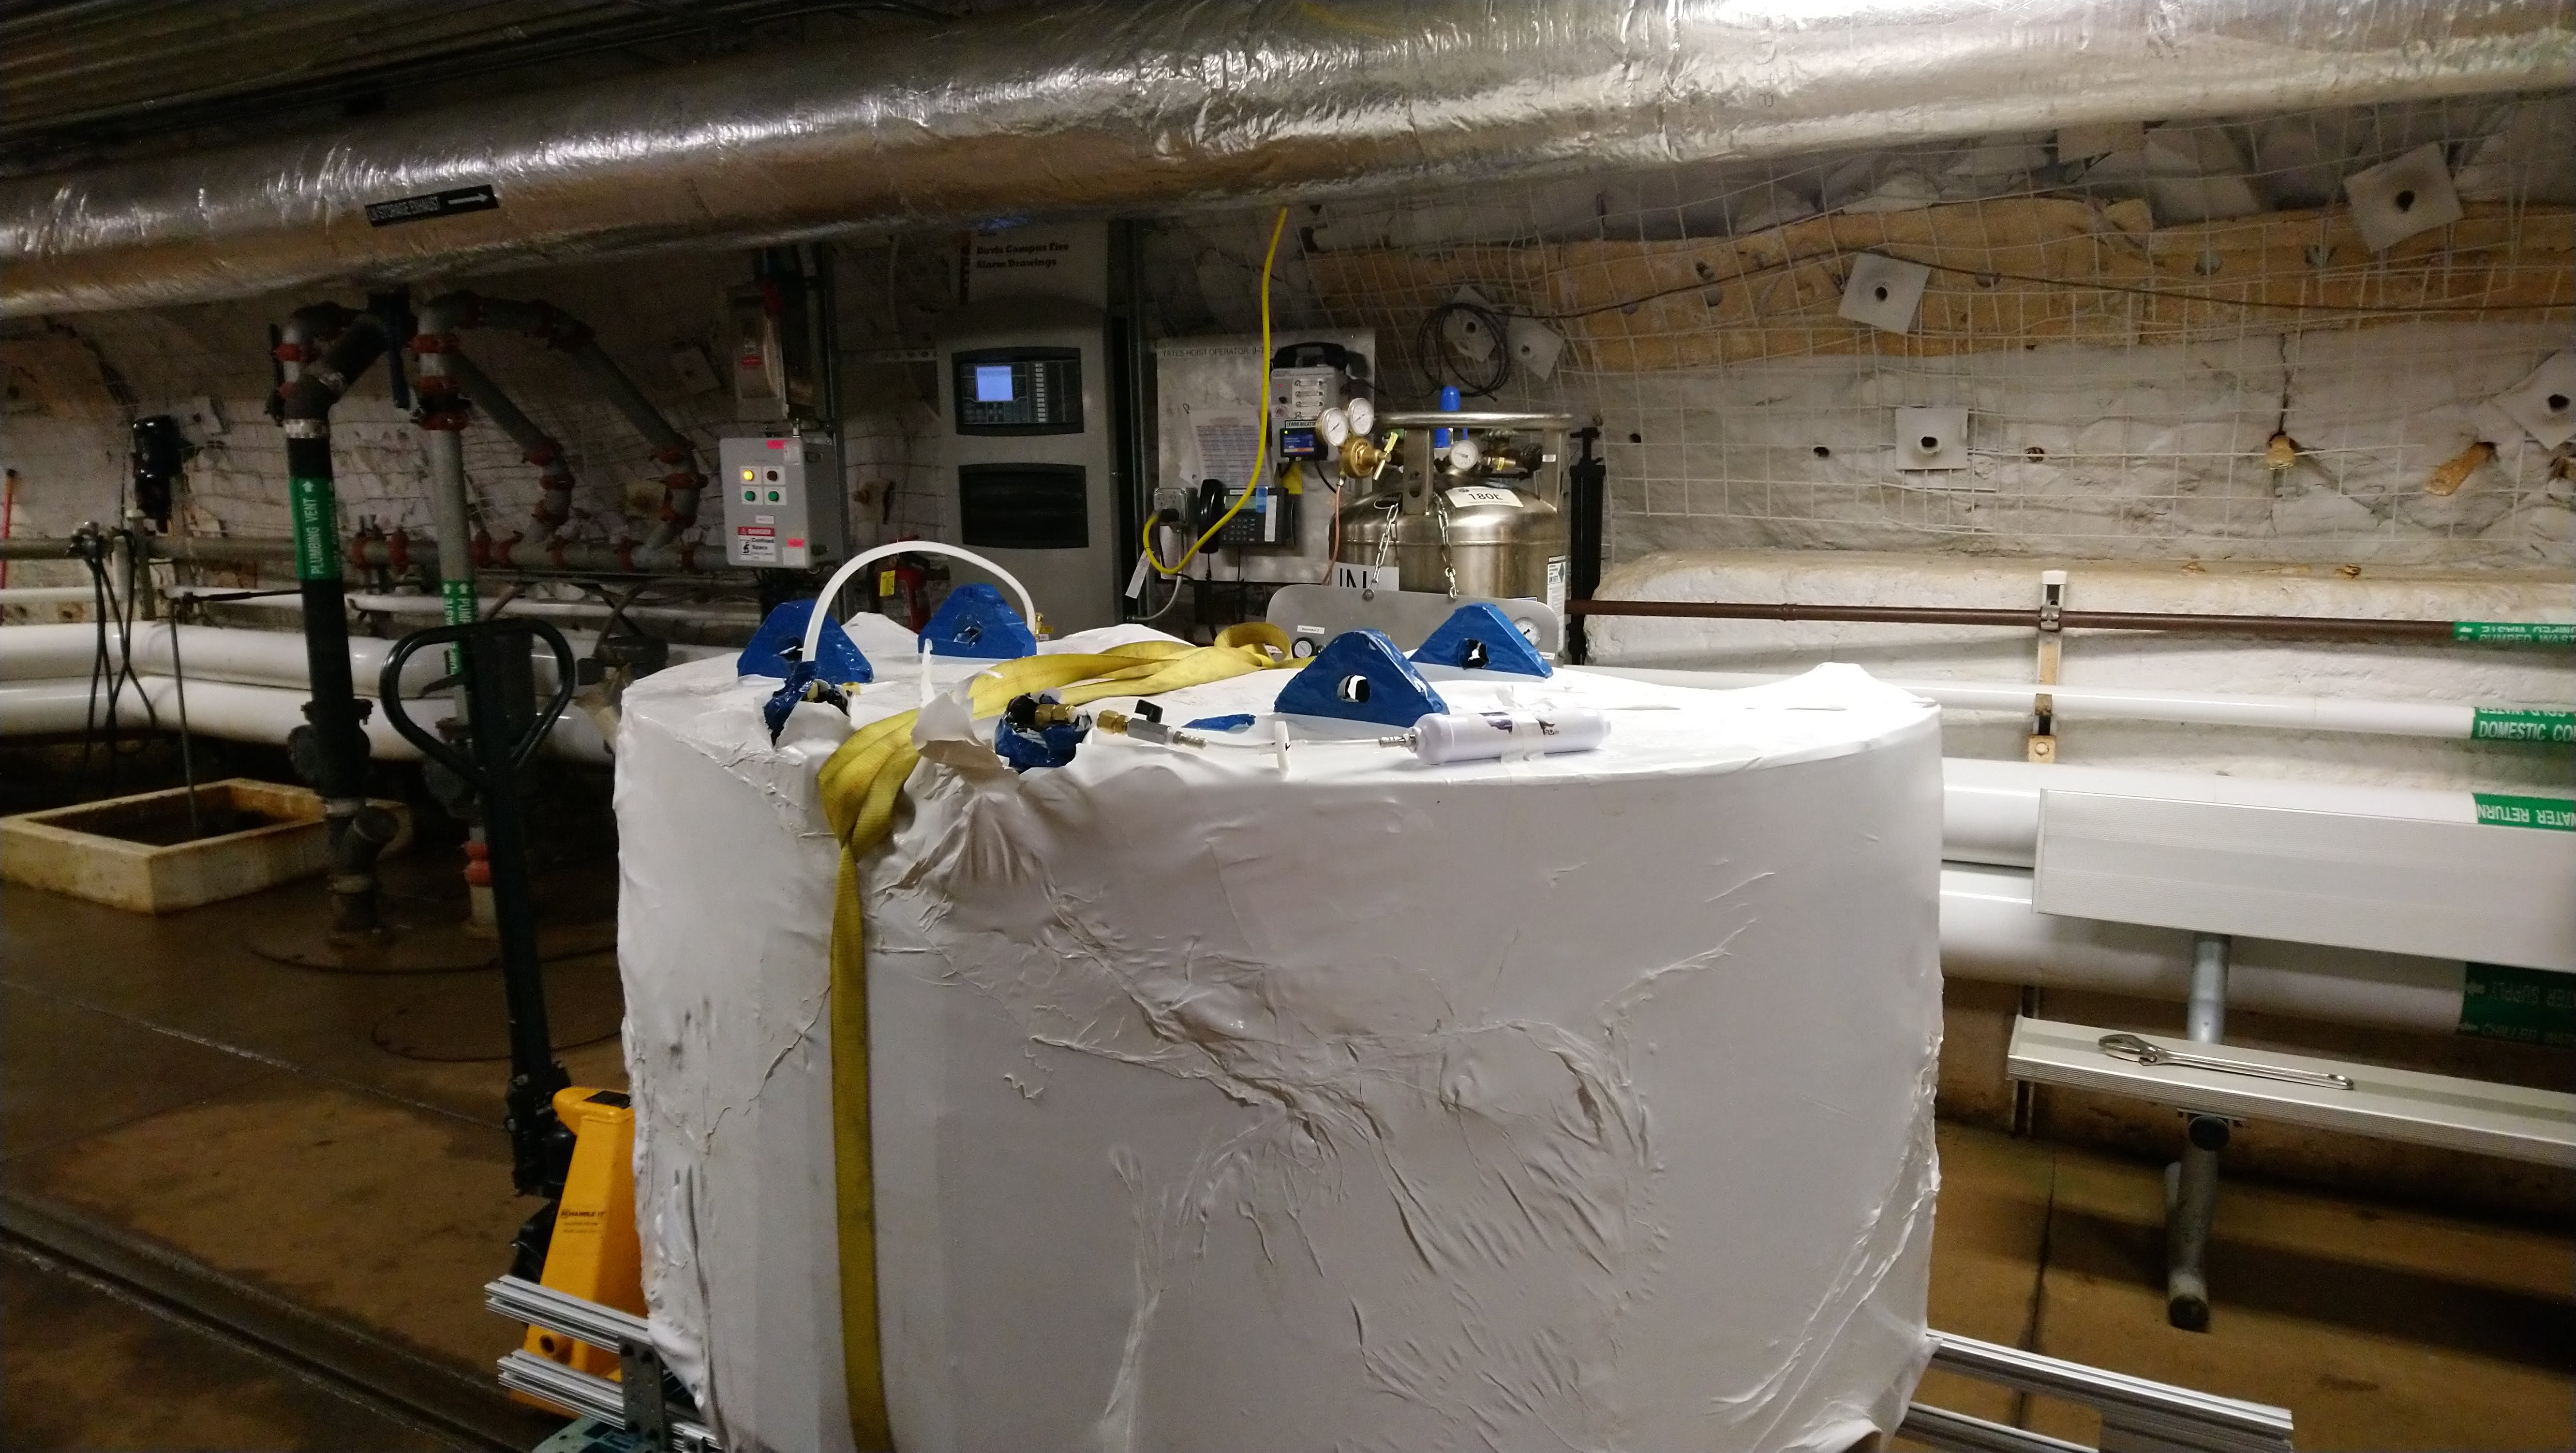
\includegraphics[width=\textwidth]{Figures/Construction/tat_purging.JPG}
\centering
\caption{Photograph of the top tank setup for N$_2$ purging after being brought underground.
         N$_2$ is warmed by being passed through a bucket of water before entering the acrylic tank.}
\label{fig:TAT_purging}
\end{figure}

\par
The proposed solution was to `correct the curvature' with foam installed on top of the OCV, which due to construction delays and COVID-19, did not begin until August 2020.
The foam used for this was Styrodur\textsuperscript{\textregistered} \cite{styrodur_foam_ref}.
This was chosen as it has a high compression strength.
It also had the benefit of being onsite as it was already planned to be used around the side tanks and was assayed in \cite{LZ_assay_ref}. 
The primary bonding method used to secure the foam to the top of the OCV was HandiFoam\textsuperscript{\textregistered} \cite{handifoam_ref}.
HandiFoam\textsuperscript{\textregistered} was chosen as it securely held test pieces together but also would fill in any potential gaps.
Additionally, the foam was held in place with titanium pins and titanium rods.
Part of the installation is shown in \autoref{fig:TAT_foam_installation}.

\begin{figure}[]
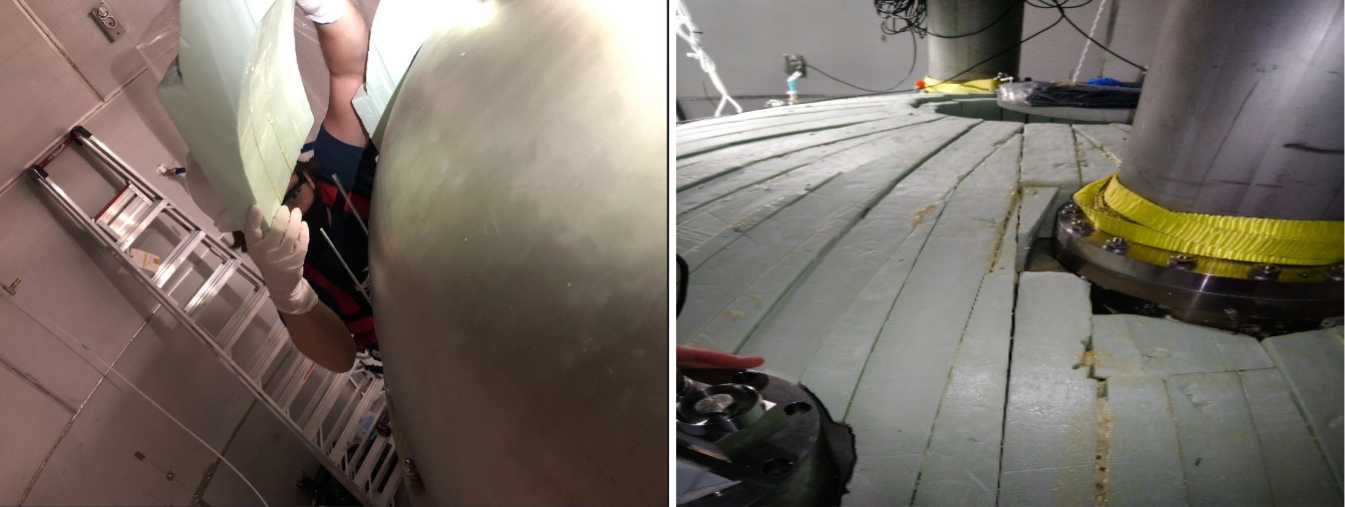
\includegraphics[width=\linewidth]{Figures/Construction/TAT_foam_installation_merged_images.png}
%\begin{subfigure}{.5\textwidth}
%  \centering
%  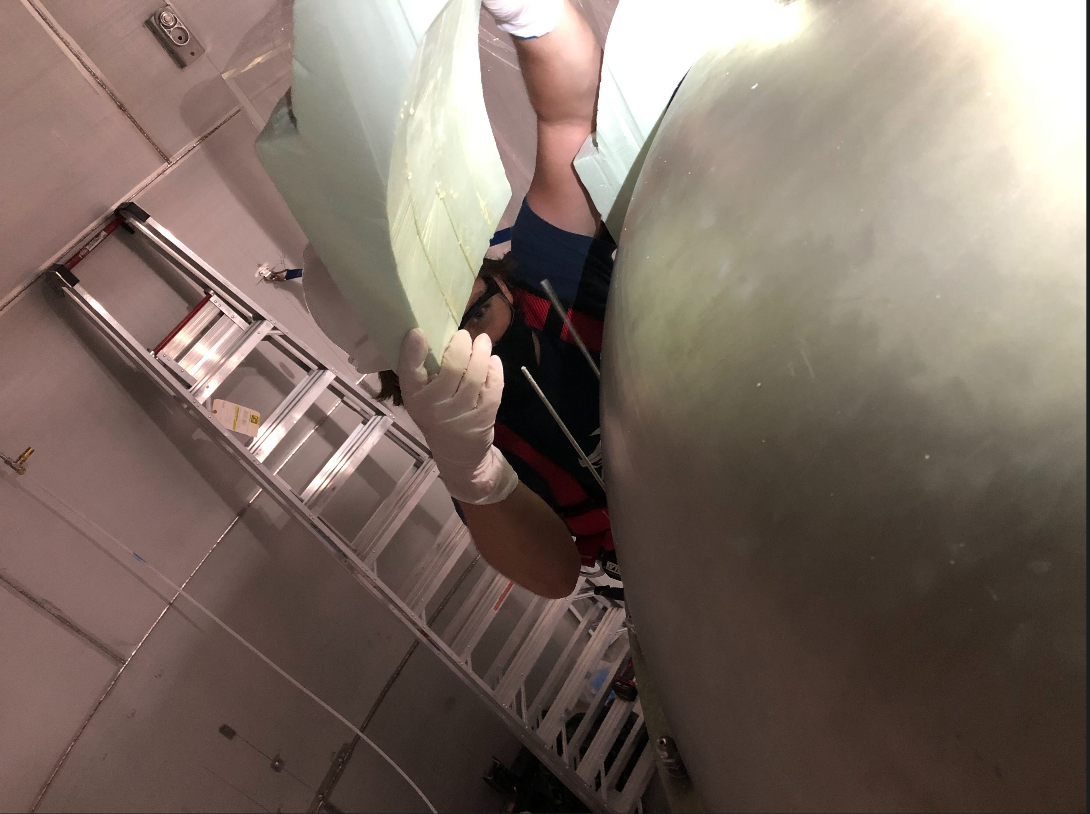
\includegraphics[height=6cm, width=\linewidth]{Figures/Construction/TAT_foam_installation.png}
%  \end{subfigure}
%  \begin{subfigure}{.5\textwidth}
%  \centering
%  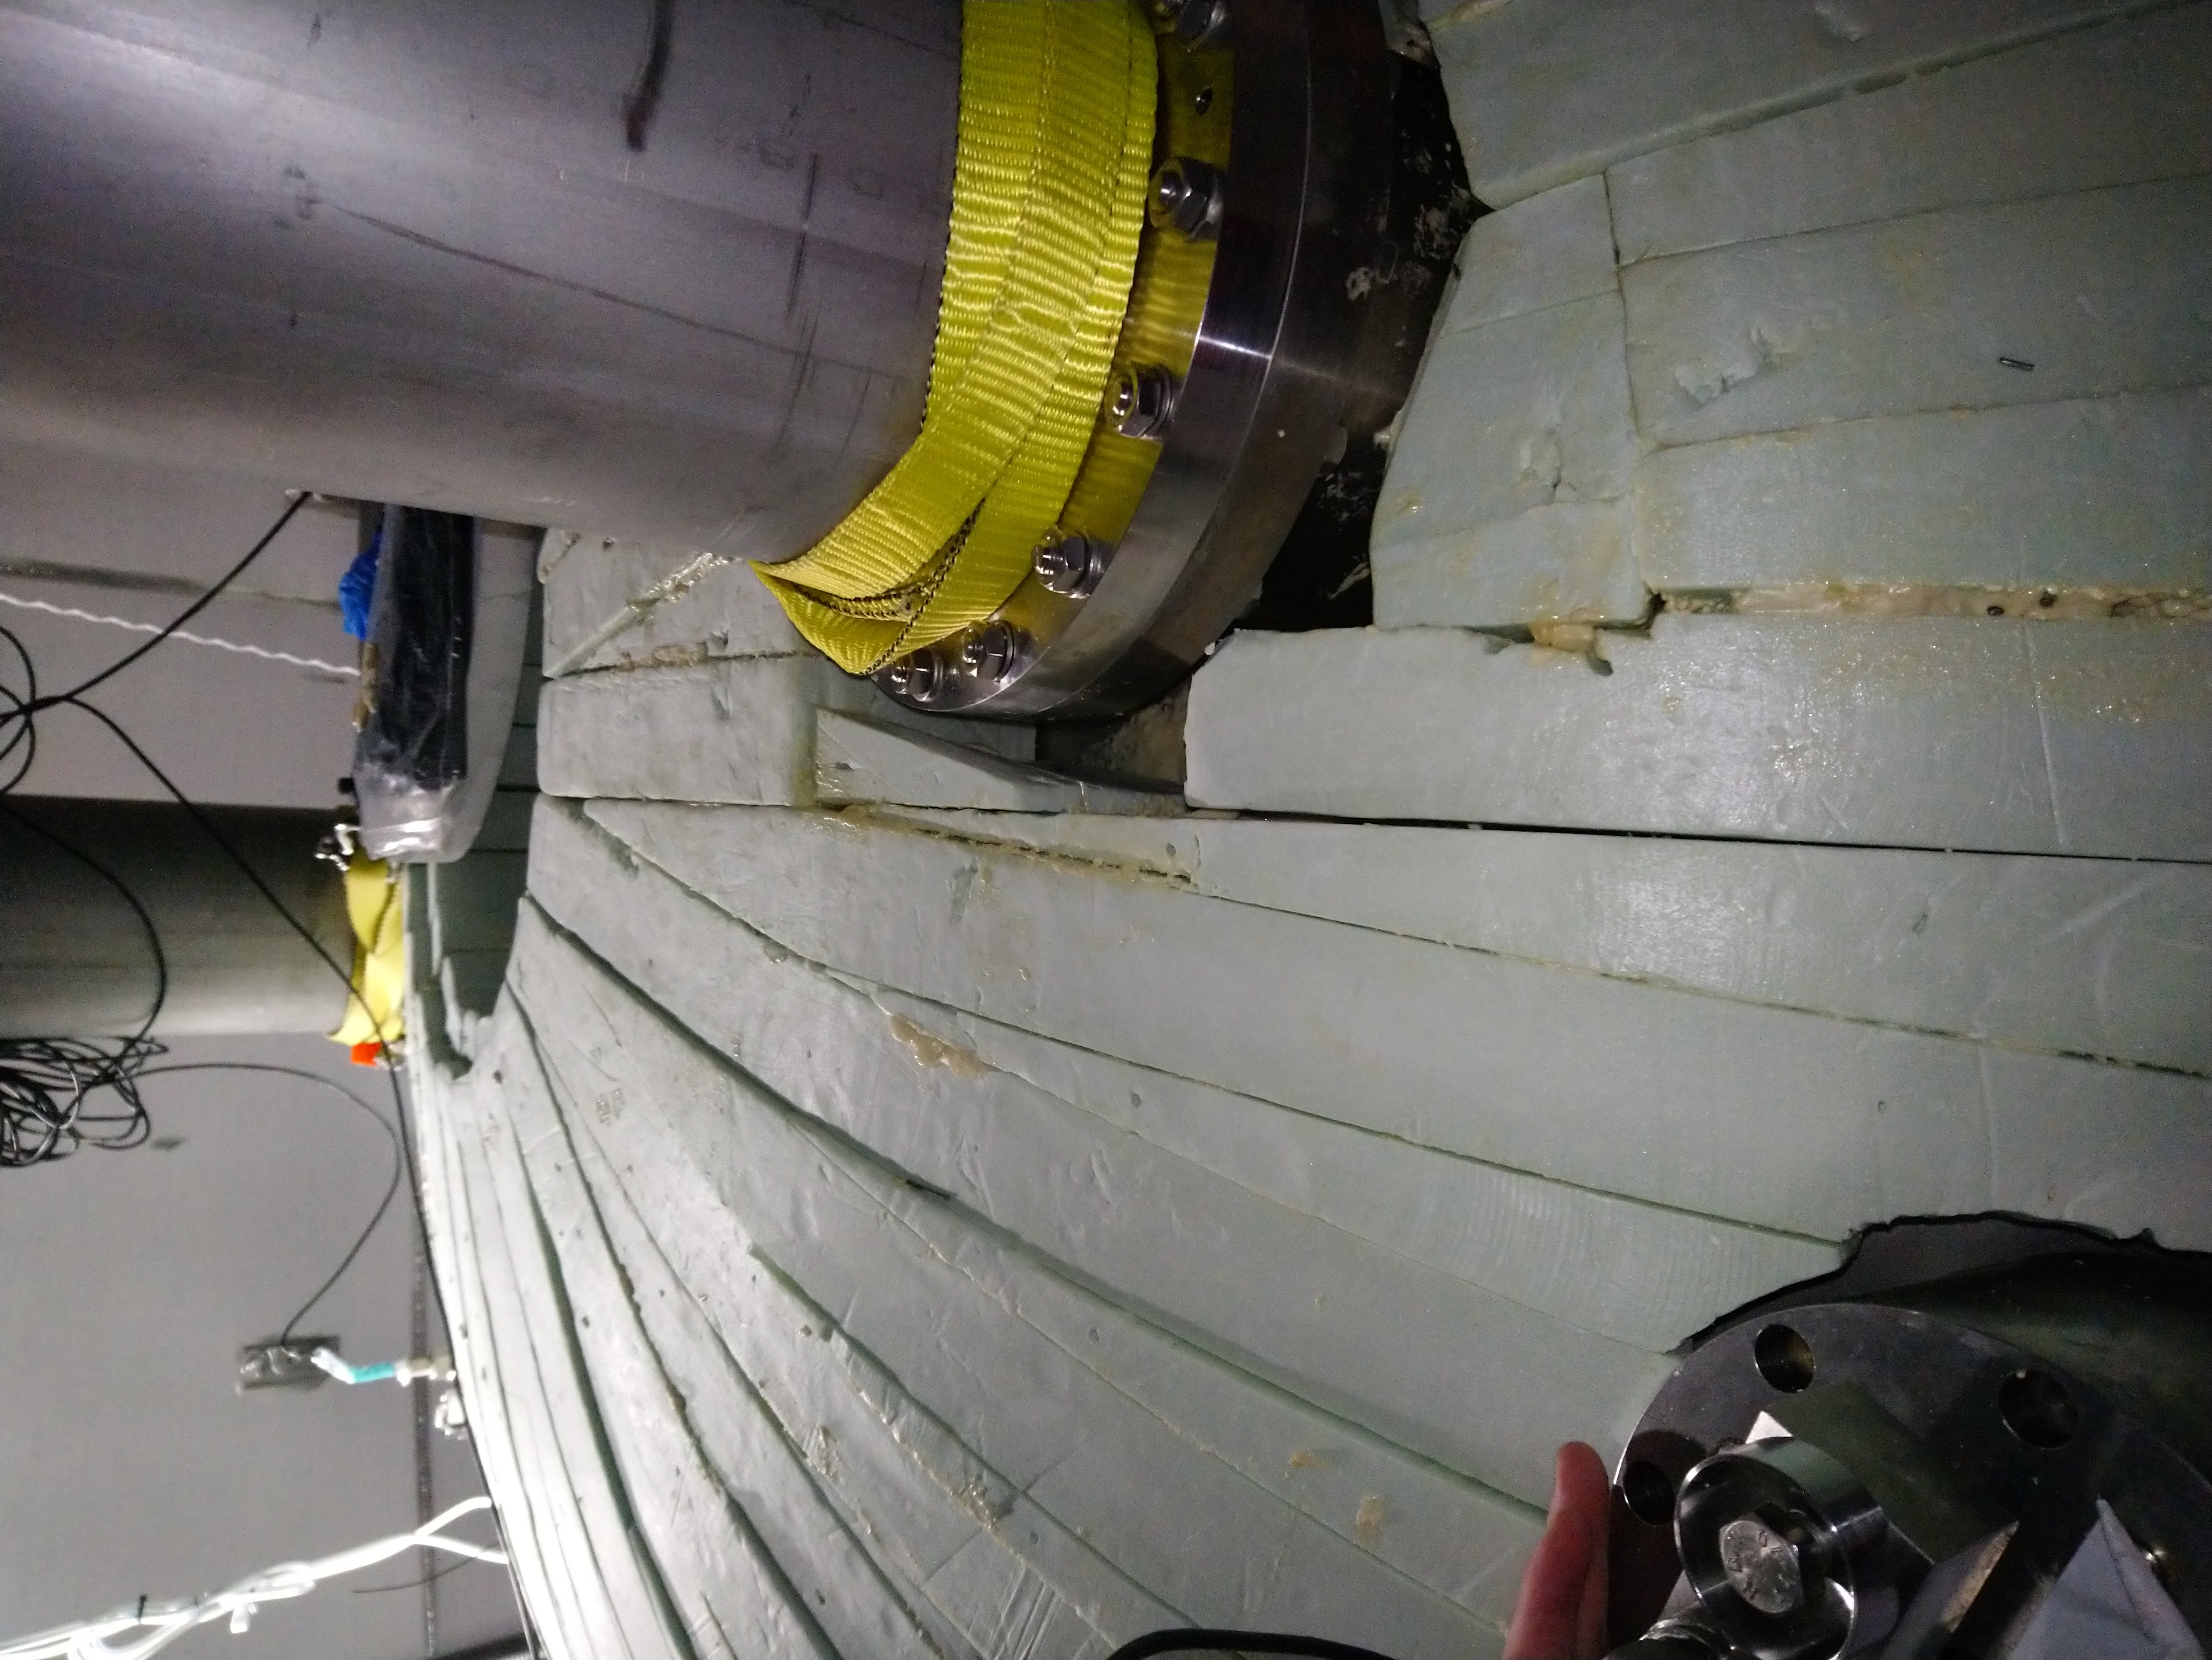
\includegraphics[height=\linewidth, width=6cm, angle=-90,]{Figures/Construction/TAT_foam_complete.jpg}
%  \end{subfigure}
\caption{Photograph of TAT-OCV foam installation.}
\label{fig:TAT_foam_installation}
\end{figure}

\par
The SAT-OCV foam was installed after the TAT-OCV foam in a slightly different fashion.
These pieces were primarily secured to each other and to the OCV using silicon sealant \cite{dowsil_silicone_ref}.
Titanium pins were also used to secure pieces together and to the bolts on the OCV.
The final fit-test is shown in \autoref{fig:sat_foam_fit_test} along with the primary OD installers.

\par
As the foam had been underground for a number of weeks prior to being used, radon chain particles are likely to have embedded themselves in each piece of foam.
To remove this, each piece of foam installed underwent a final `shaving', where a few mm was removed from each side.
This is shown in \autoref{fig:sat_foam_shaving}.

\begin{figure}[]
  \begin{subfigure}{.5\textwidth}
  \centering
  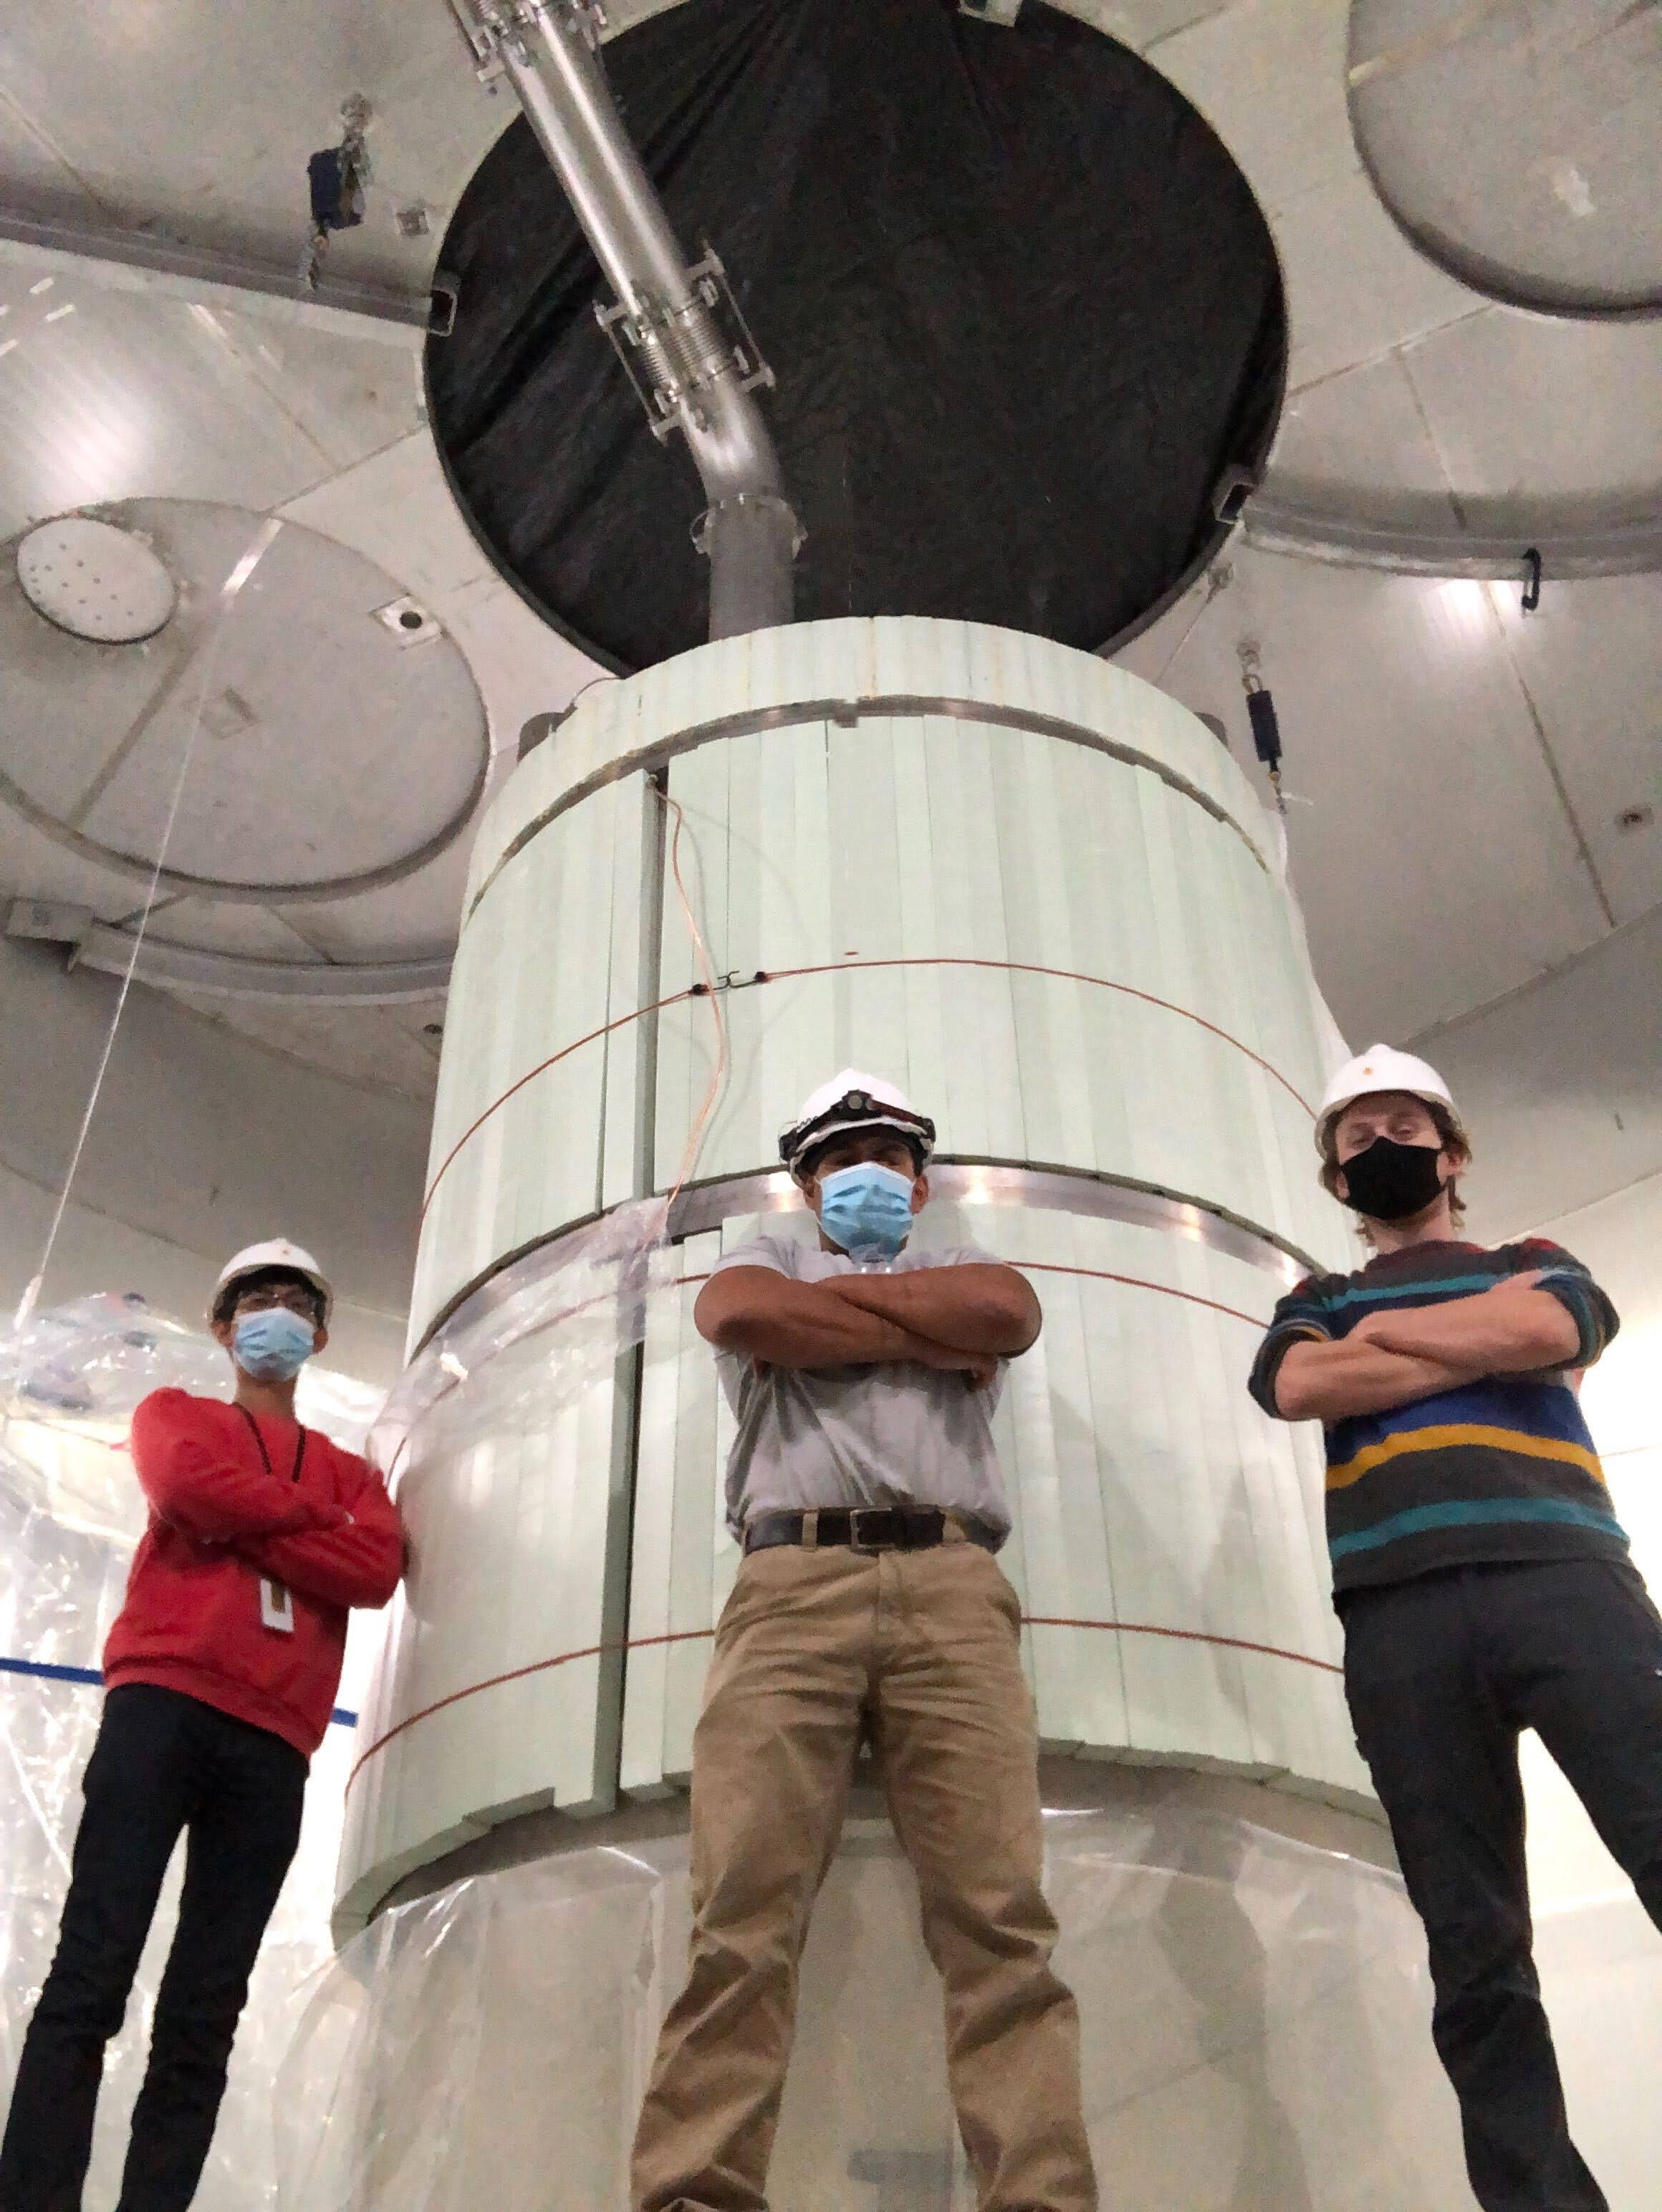
\includegraphics[width=\linewidth]{Figures/Construction/SAT_foam_fittest.jpg}
  \caption{OCV side foam test fit along with the primary OD installers}
  \label{fig:sat_foam_fit_test}
  \end{subfigure}
  \begin{subfigure}{.5\textwidth}
  \centering
  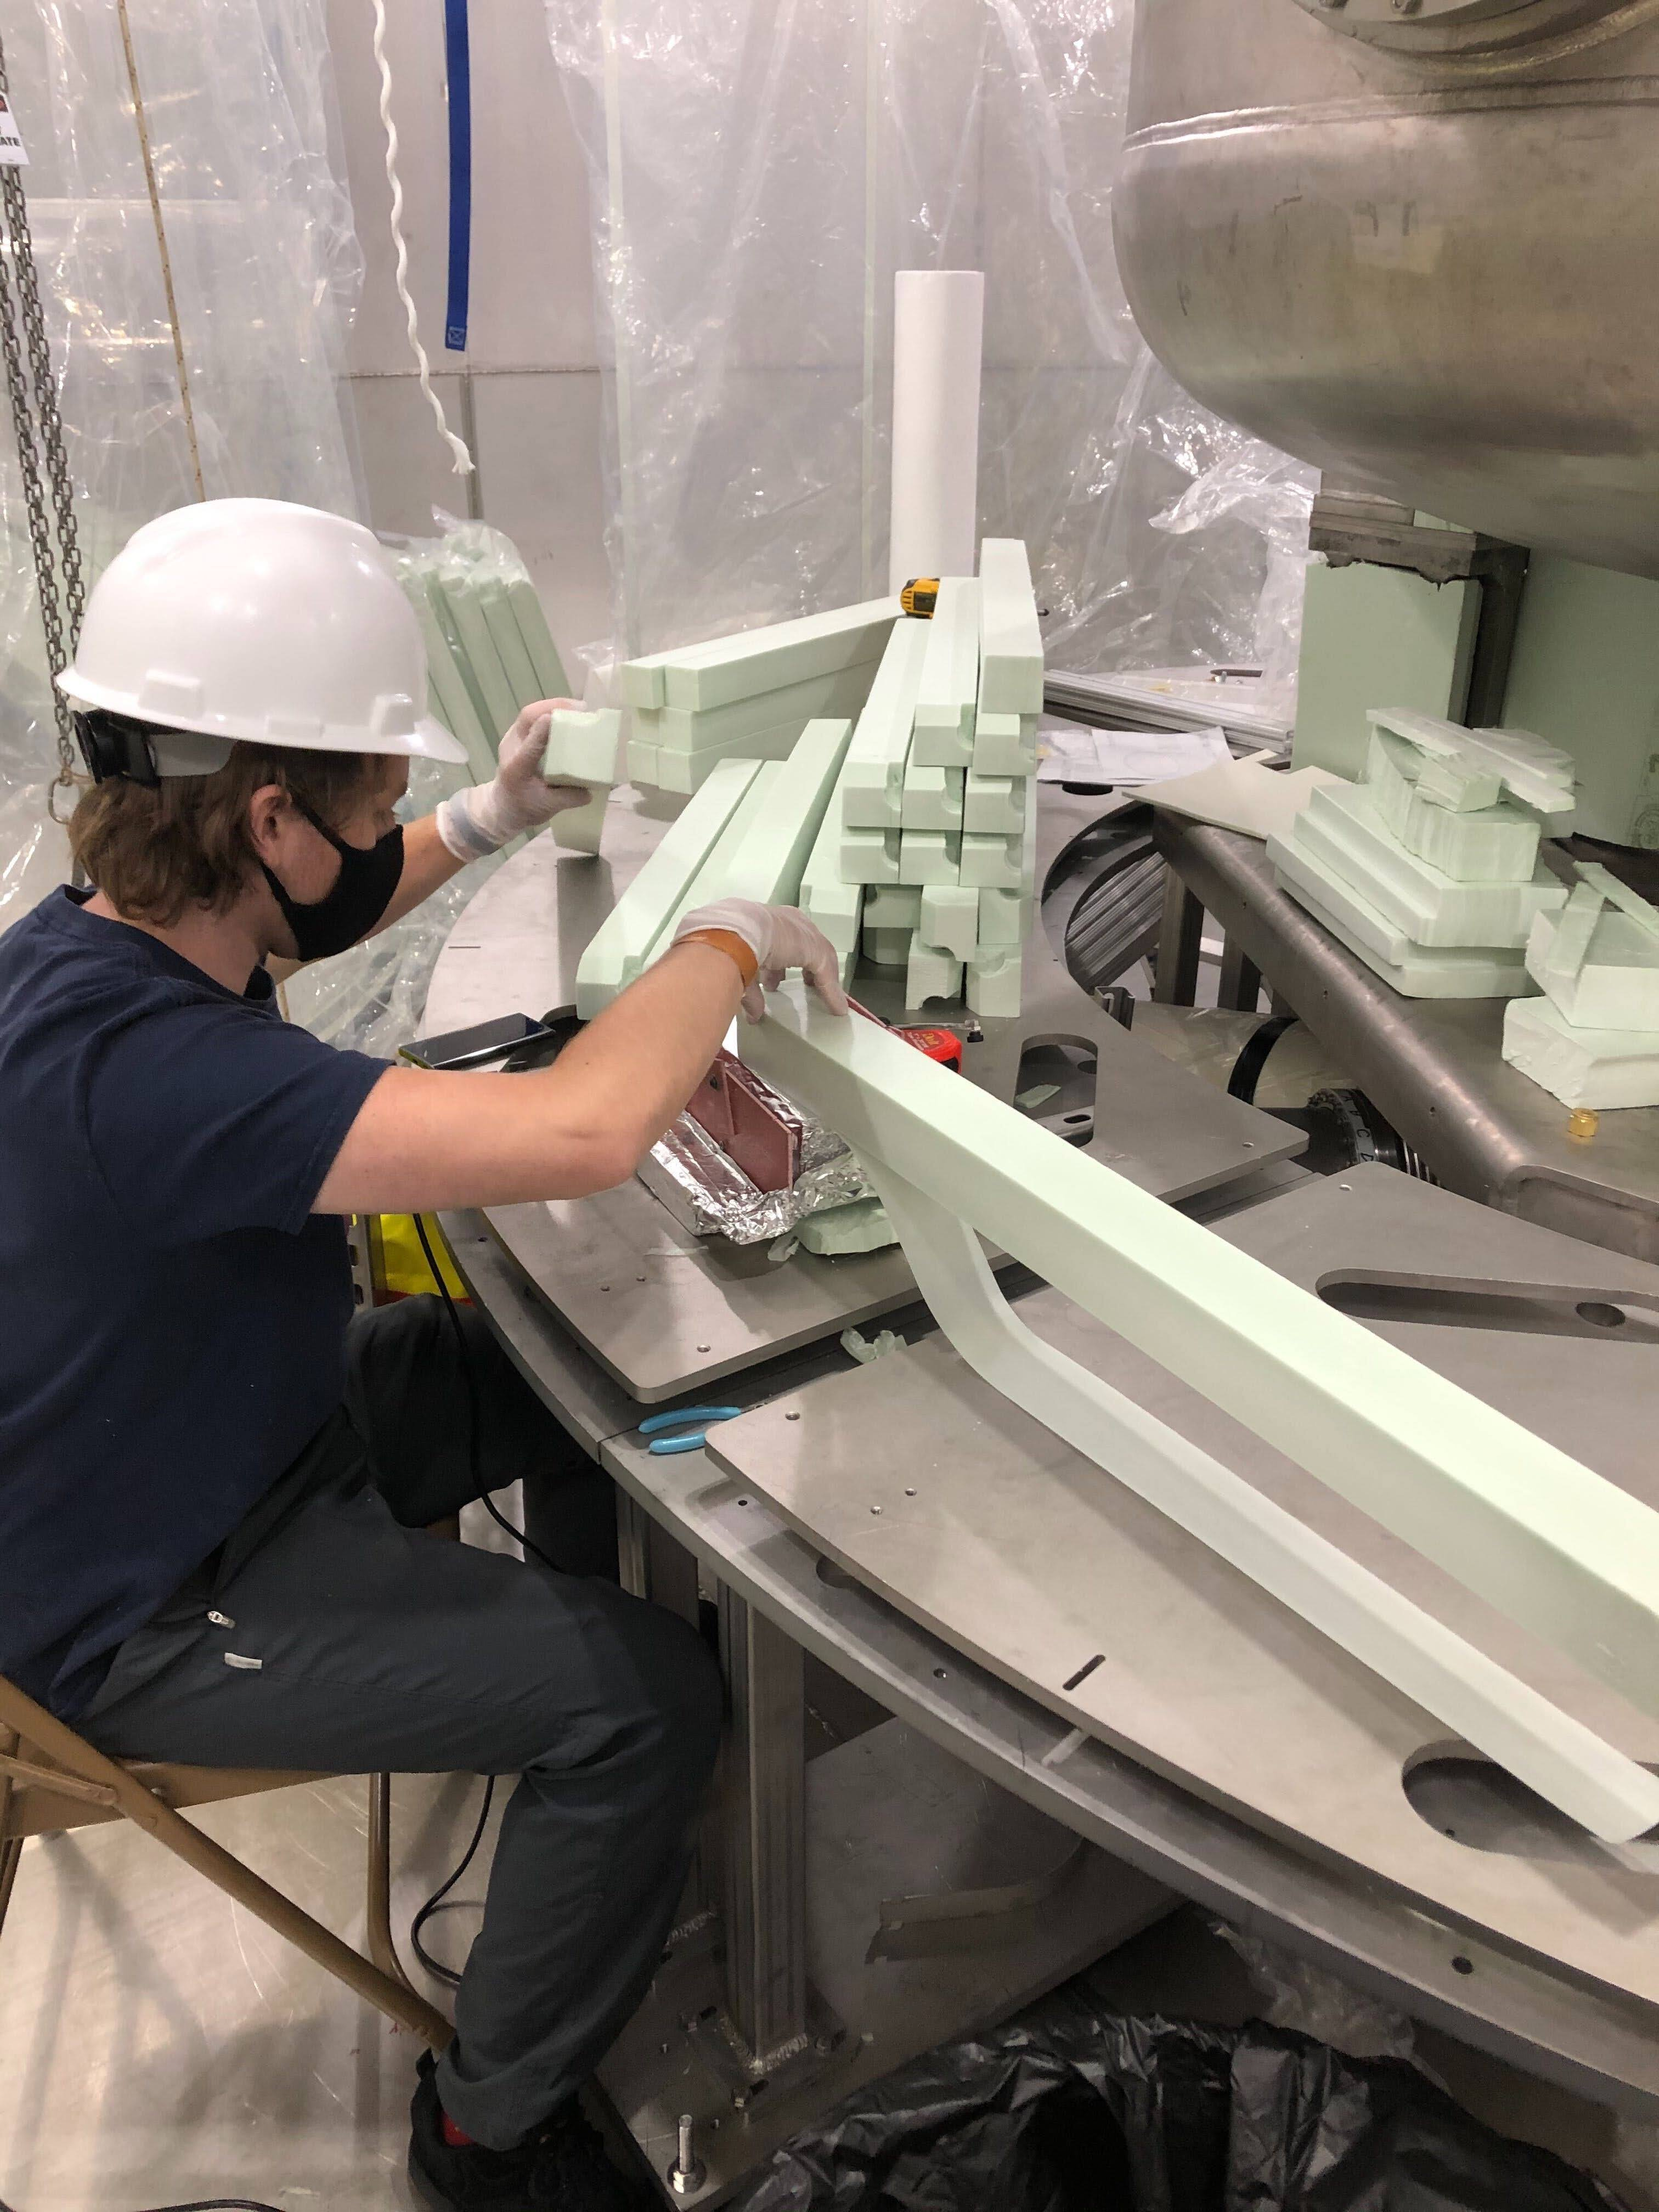
\includegraphics[width=\linewidth]{Figures/Construction/foam_shaving.jpg}
  \caption{Author using hot-knife to shave all SAT foam prior to installation}
  \label{fig:sat_foam_shaving}
  \end{subfigure}
\caption{Photographs of SAT-OCV foam installation.}
\label{fig:SAT_foam_installation}
\end{figure}

\par
Additionally, the foam was installed around the OCV legs in between the BATs.
This foam was secured using HandiFoam\textsuperscript{\textregistered} as shown in \autoref{fig:ocv_leg_foam}.

\begin{figure}[!tbph]
%\centering
%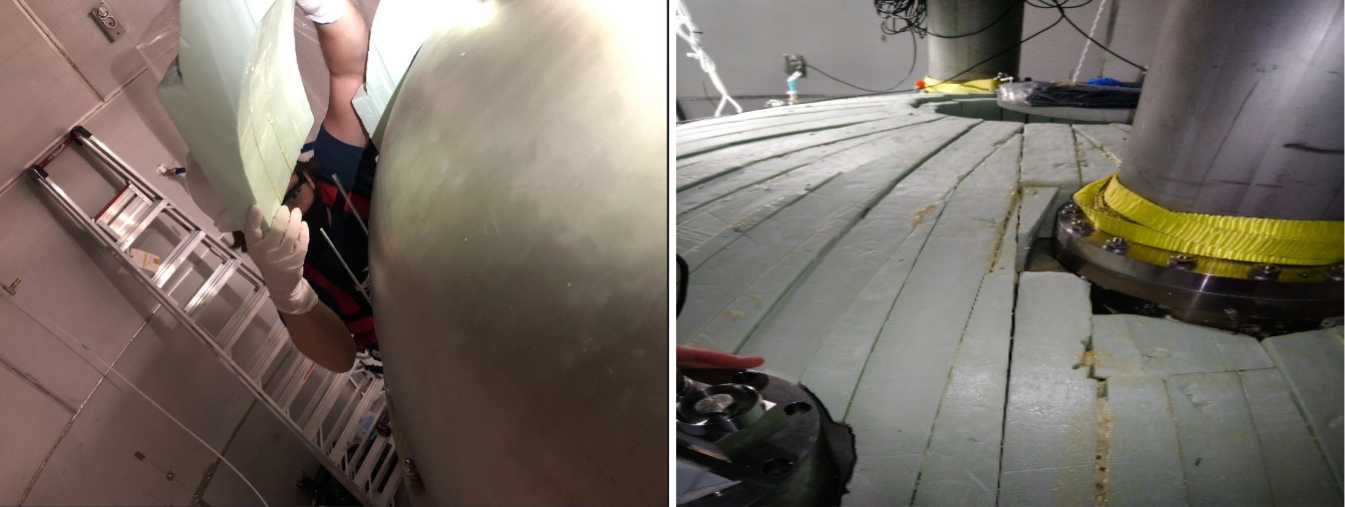
\includegraphics[width=\linewidth]{Figures/Construction/TAT_foam_installation_merged_images.png}
\begin{subfigure}{.5\textwidth}
  \centering
  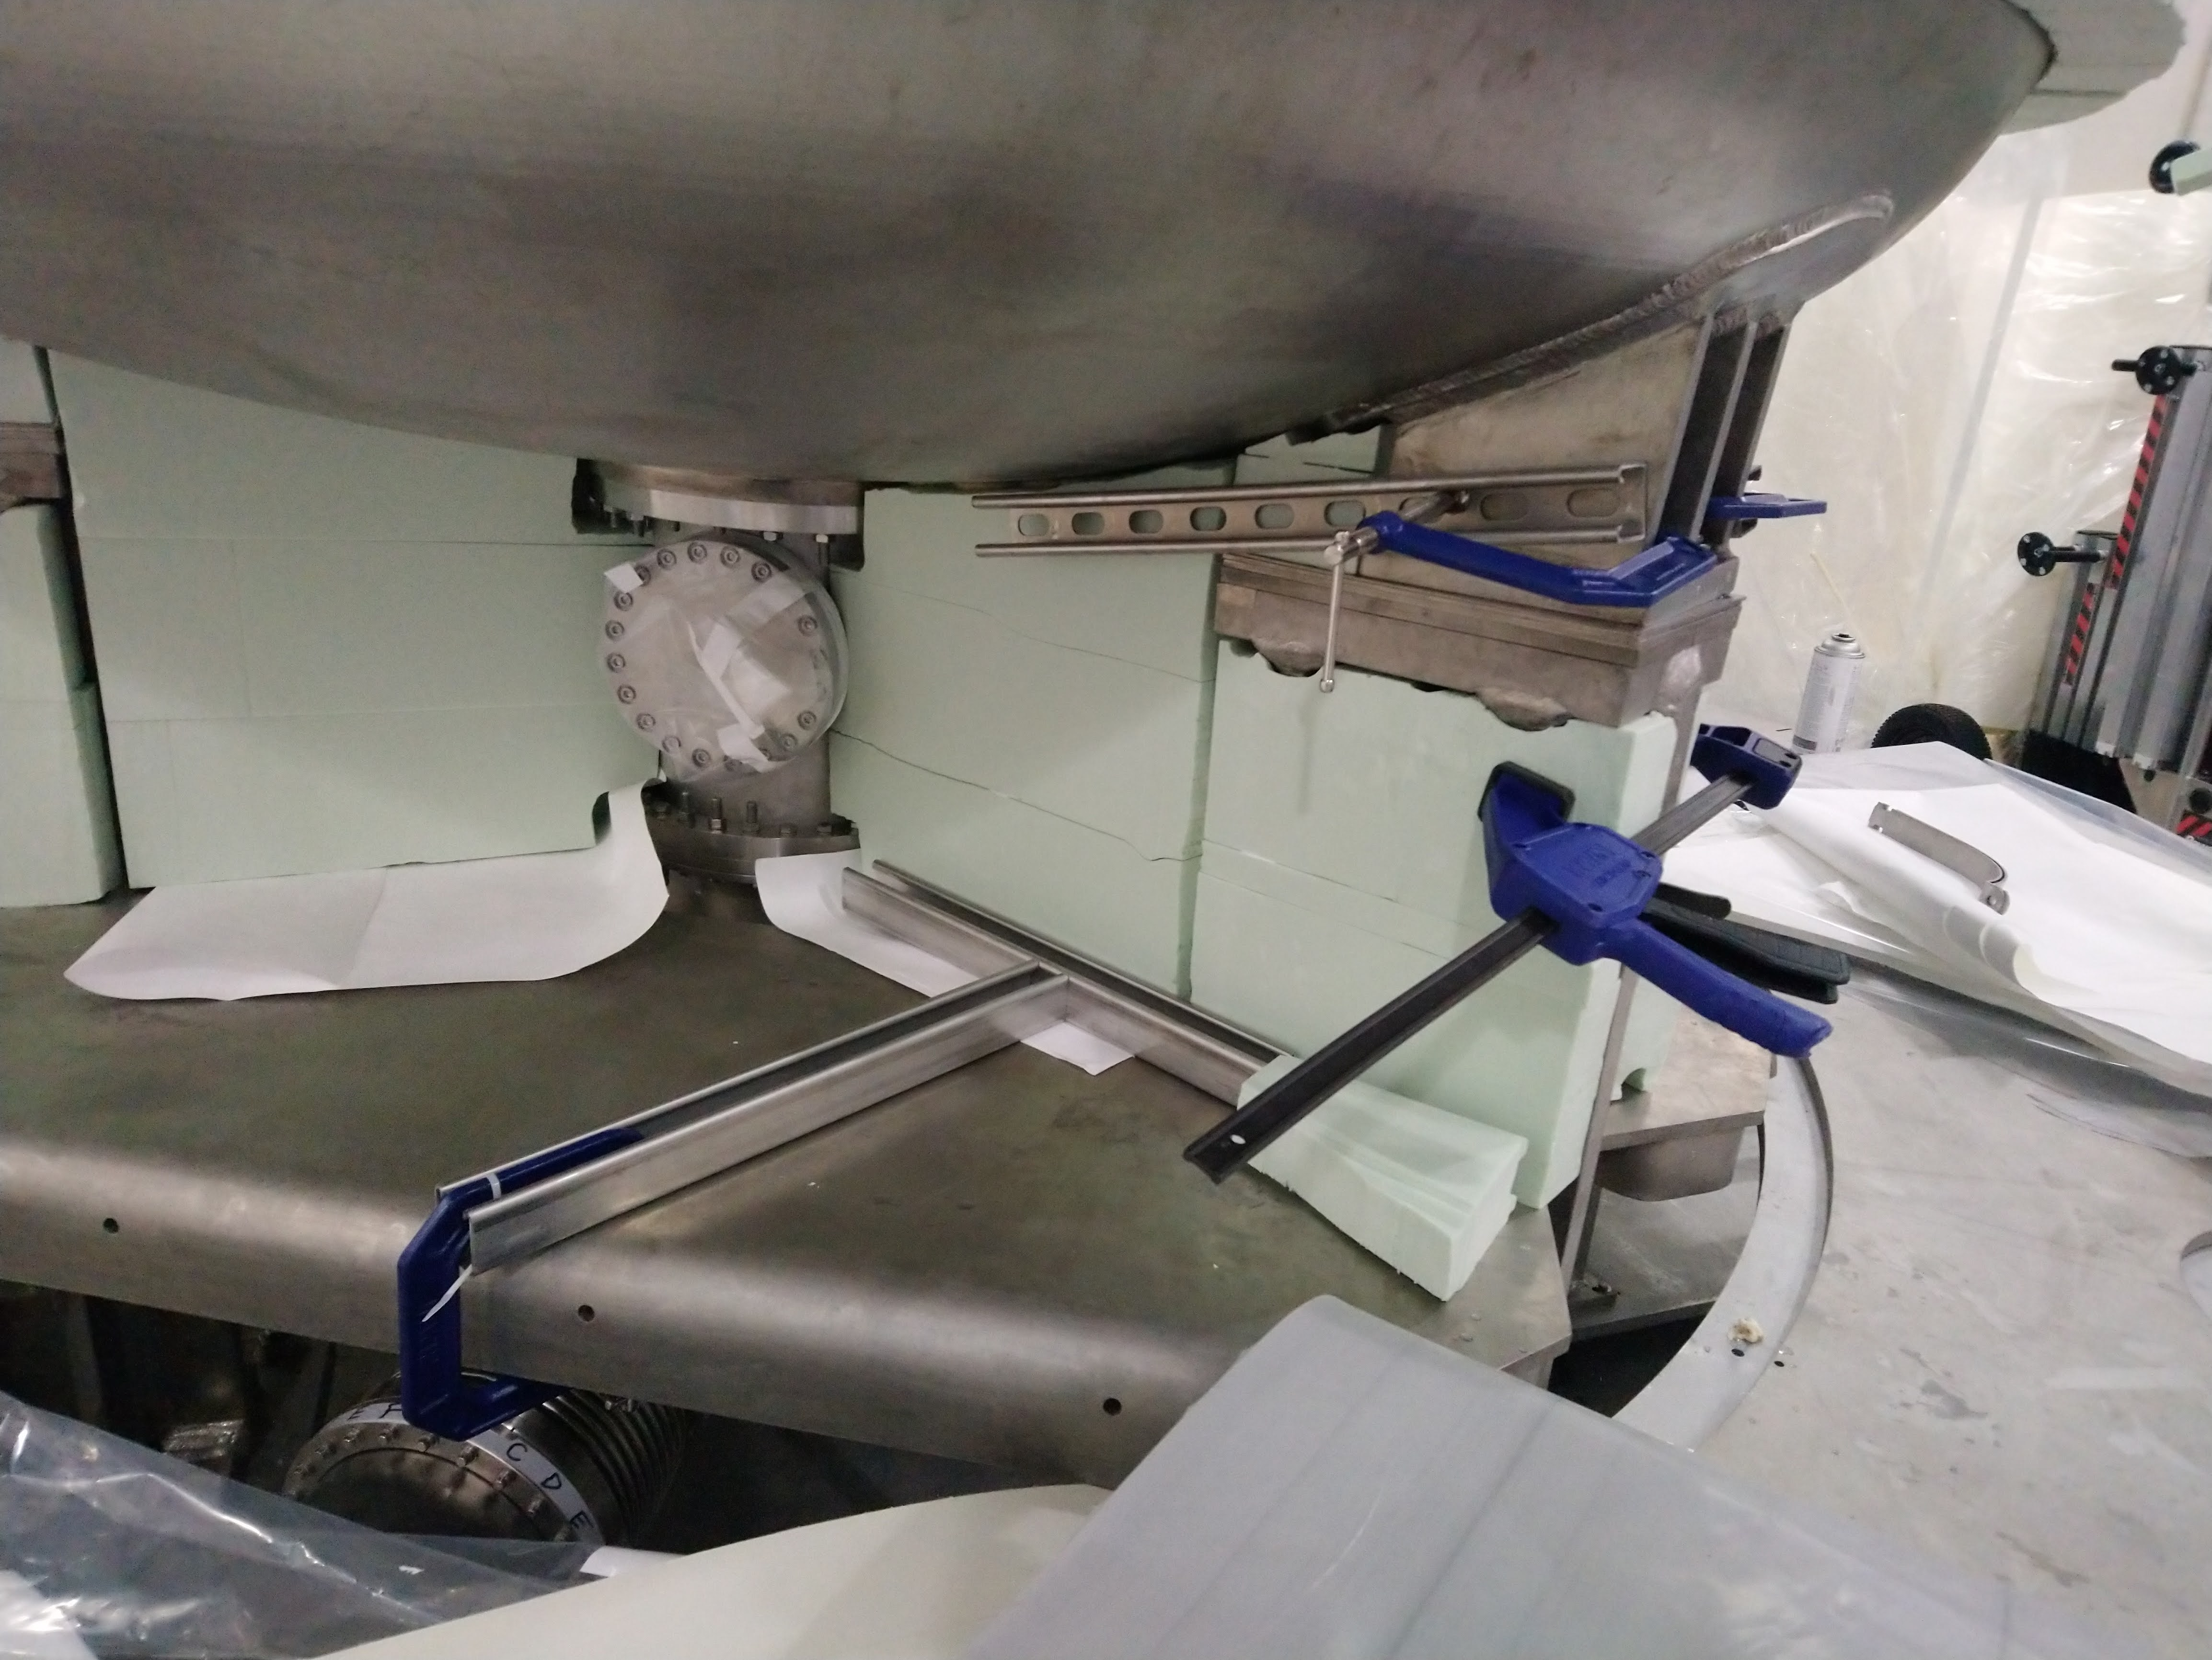
\includegraphics[height=6cm, width=\linewidth]{Figures/Construction/BAT_green_foam.JPG}
  \caption{OVV leg foam installation.}
  \label{fig:ocv_leg_foam}
  \end{subfigure}
  \begin{subfigure}{.5\textwidth}
  \centering
  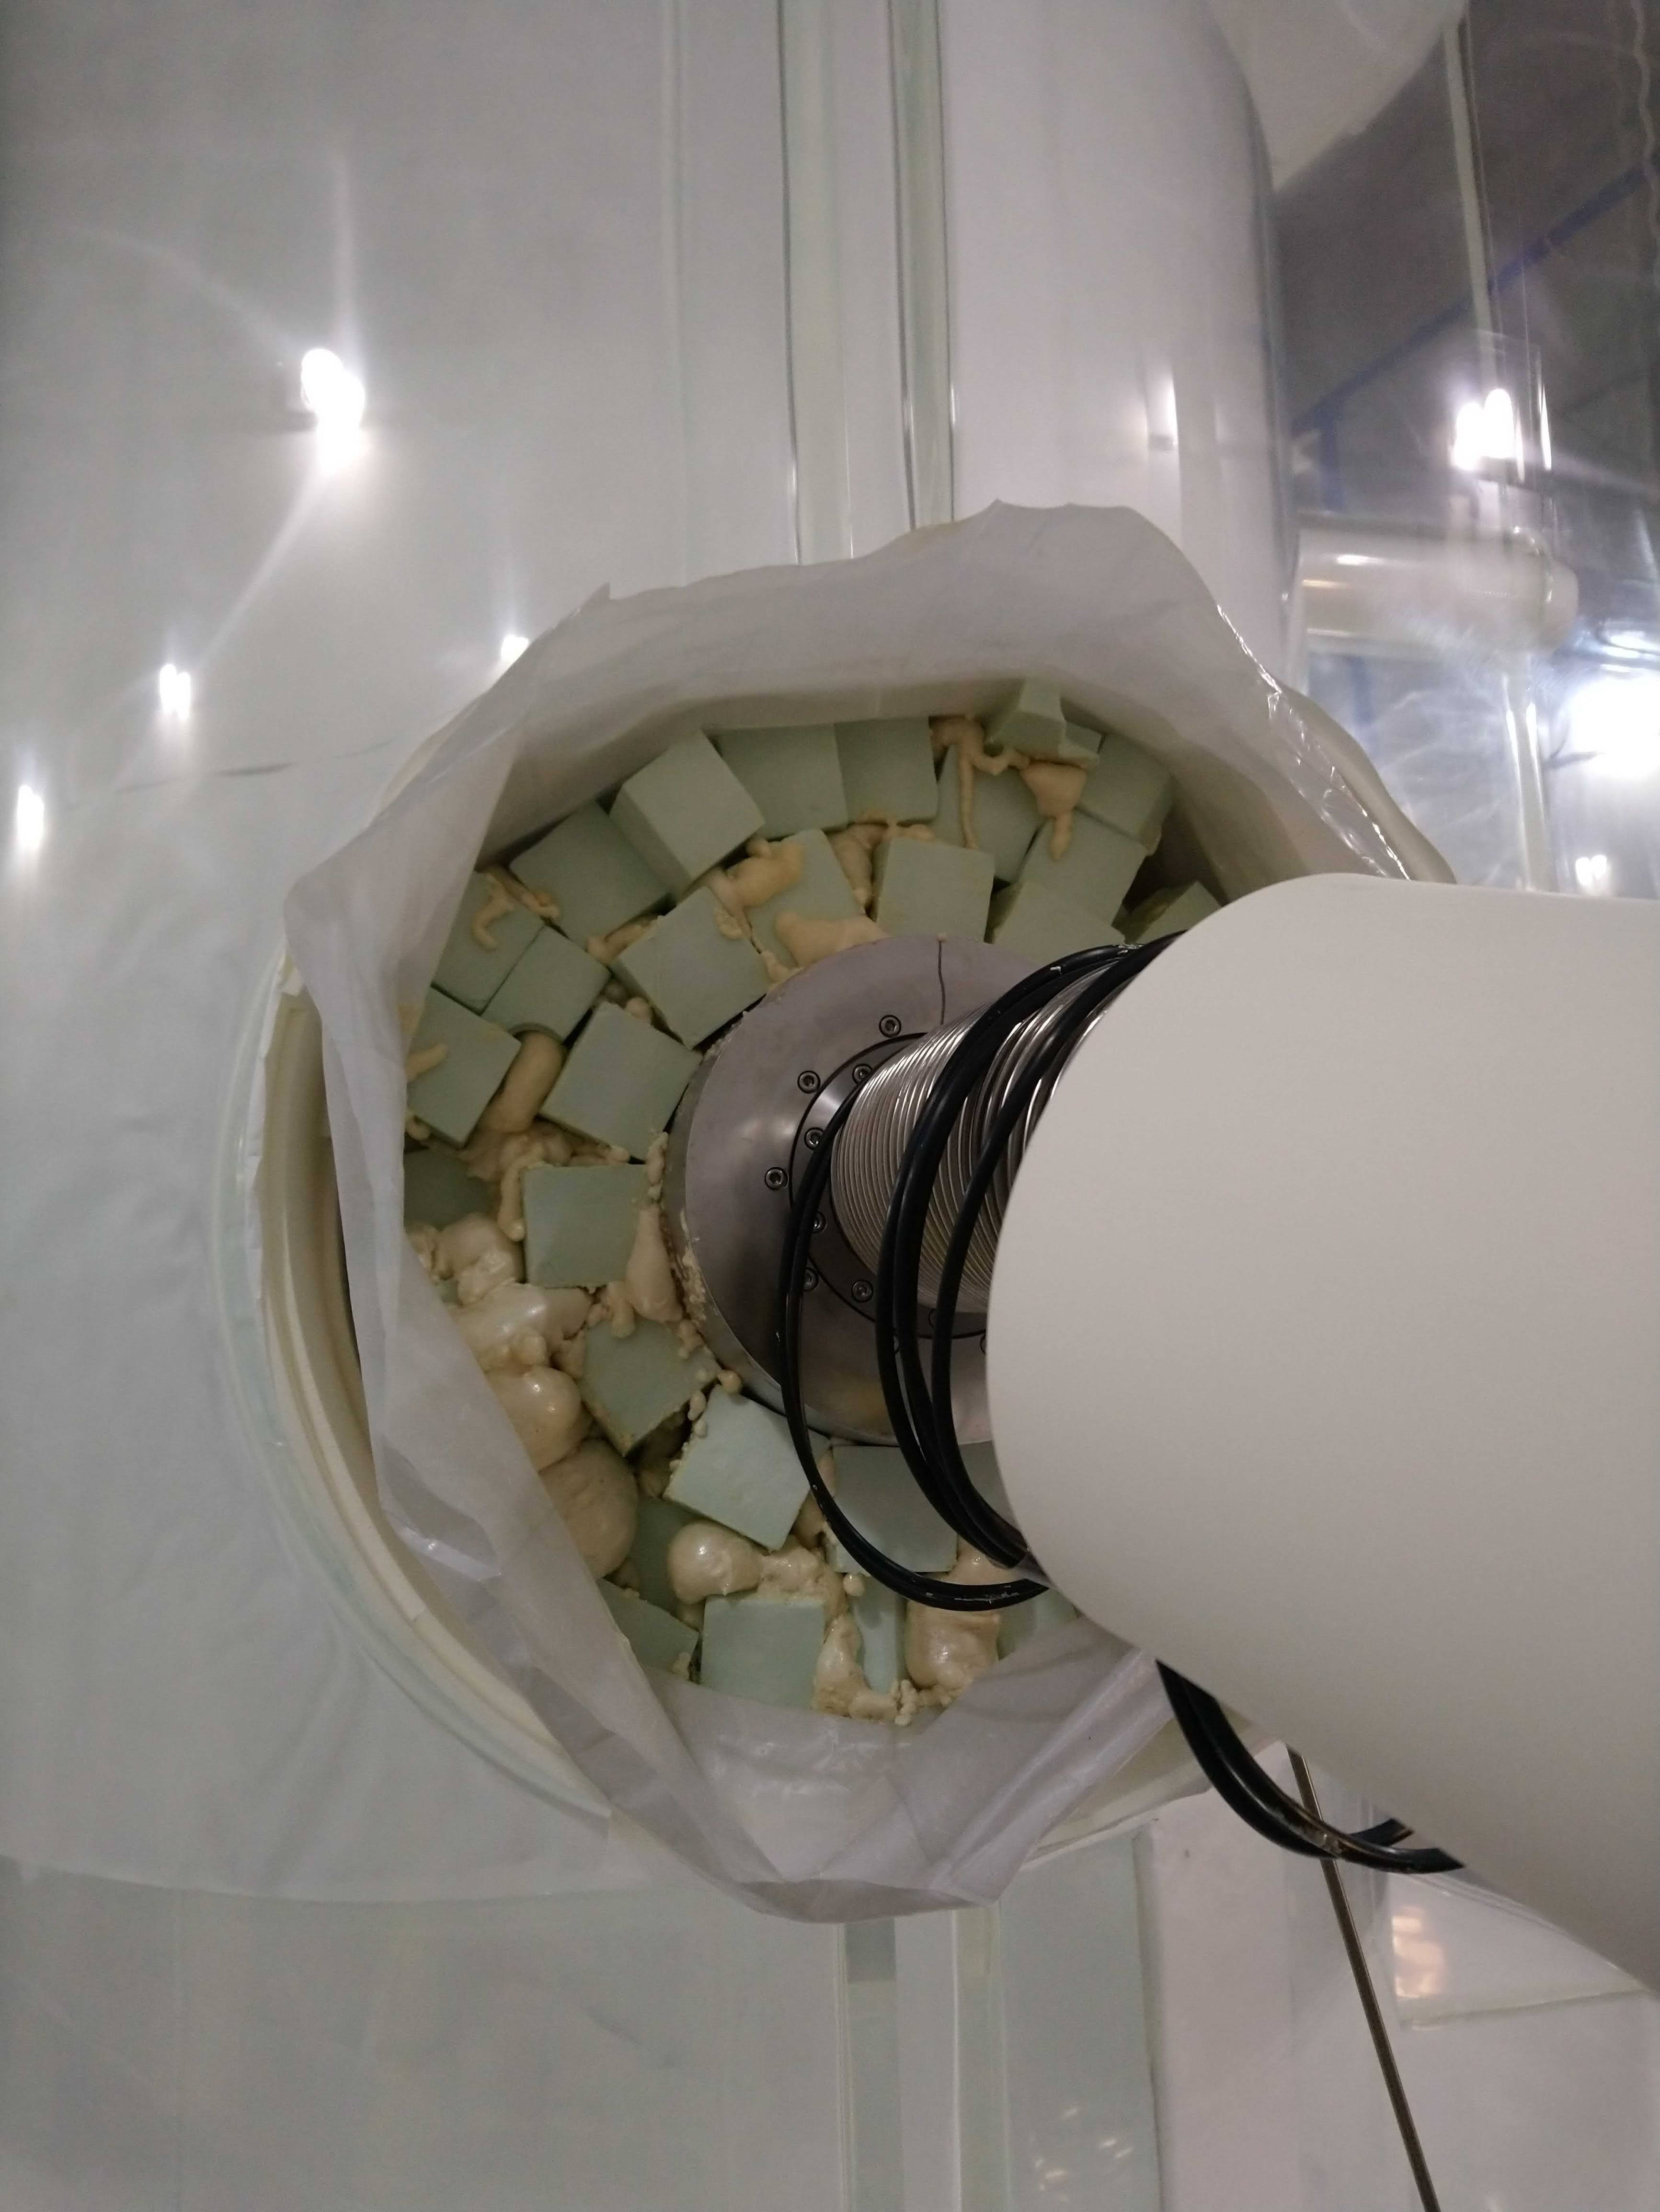
\includegraphics[height=6cm, width=\linewidth]{Figures/Construction/HV_foam.jpg}
  \caption{Foam installed around HV-feedthrough in SATs.}
  \label{fig:hv_port_foam}
  \end{subfigure}
\caption{Photographs of foam installed around OCV and HV-feedthrough.}
\label{fig:Additional_foam_installation}
\end{figure}

\par
Because of the aforementioned split tank and thin walls, there was a danger that the tanks may leak GdLS.
This is not necessarily a problem as GdLS is oil-based, so would float to the top of the water, allowing it to be collected easily.
However, it does not react well with either Tyvek or foam, both of which surround the OCV, and so any leaking GdLS would inevitably come into contact with them.
Over long exposure, the optical reflectivity of Tyvek is damaged, reducing light collection in the OD, but it would still work to some extent.
The foam, on the other hand, would degrade sufficiently such that it would no longer serve its purpose as a water displacer after any contact.
As such, polyethylene sheets were installed to cover the foam.
On top of this, the Tyvek was installed.
In addition, the OD-Tyvek shape around the TAT was changed.
Previously this was a flat Tyvek sheet lying on top of the TAT and out to the OD PMTs.
However, in order to allow for a potential GdLS leak to reach the surface of the water, a TeePee design was adopted.
This was so that any GdLS leak could follow a path to the top of the water.

\par
During the bottom acrylic tank (BAT) test-fitting, it was found that these also did not match the curvature of the OCV.
Additionally, because of the placement of the BAT securing feet, they were unstable.
This meant that as the water tank was filled, the BATs could rock and bash into the OCV and potentially break their feet off, causing a leak.
The installation solution was to secure the BATs as much as possible with foam.
A different, thinner foam was selected for this purpose, as a degree of flexibility was required to follow the OCV curve.
In this place, 1/4-inch and 1/2-inch polyethylene foam were selected \cite{white_foam_ref}.
Additionally, HandiFoam\textsuperscript{\textregistered} was used for smaller places that could not be reached.
The final BAT installation is shown in \autoref{fig:BAT_installation}.

\begin{figure}[]
\begin{subfigure}{.5\textwidth}
  \centering
  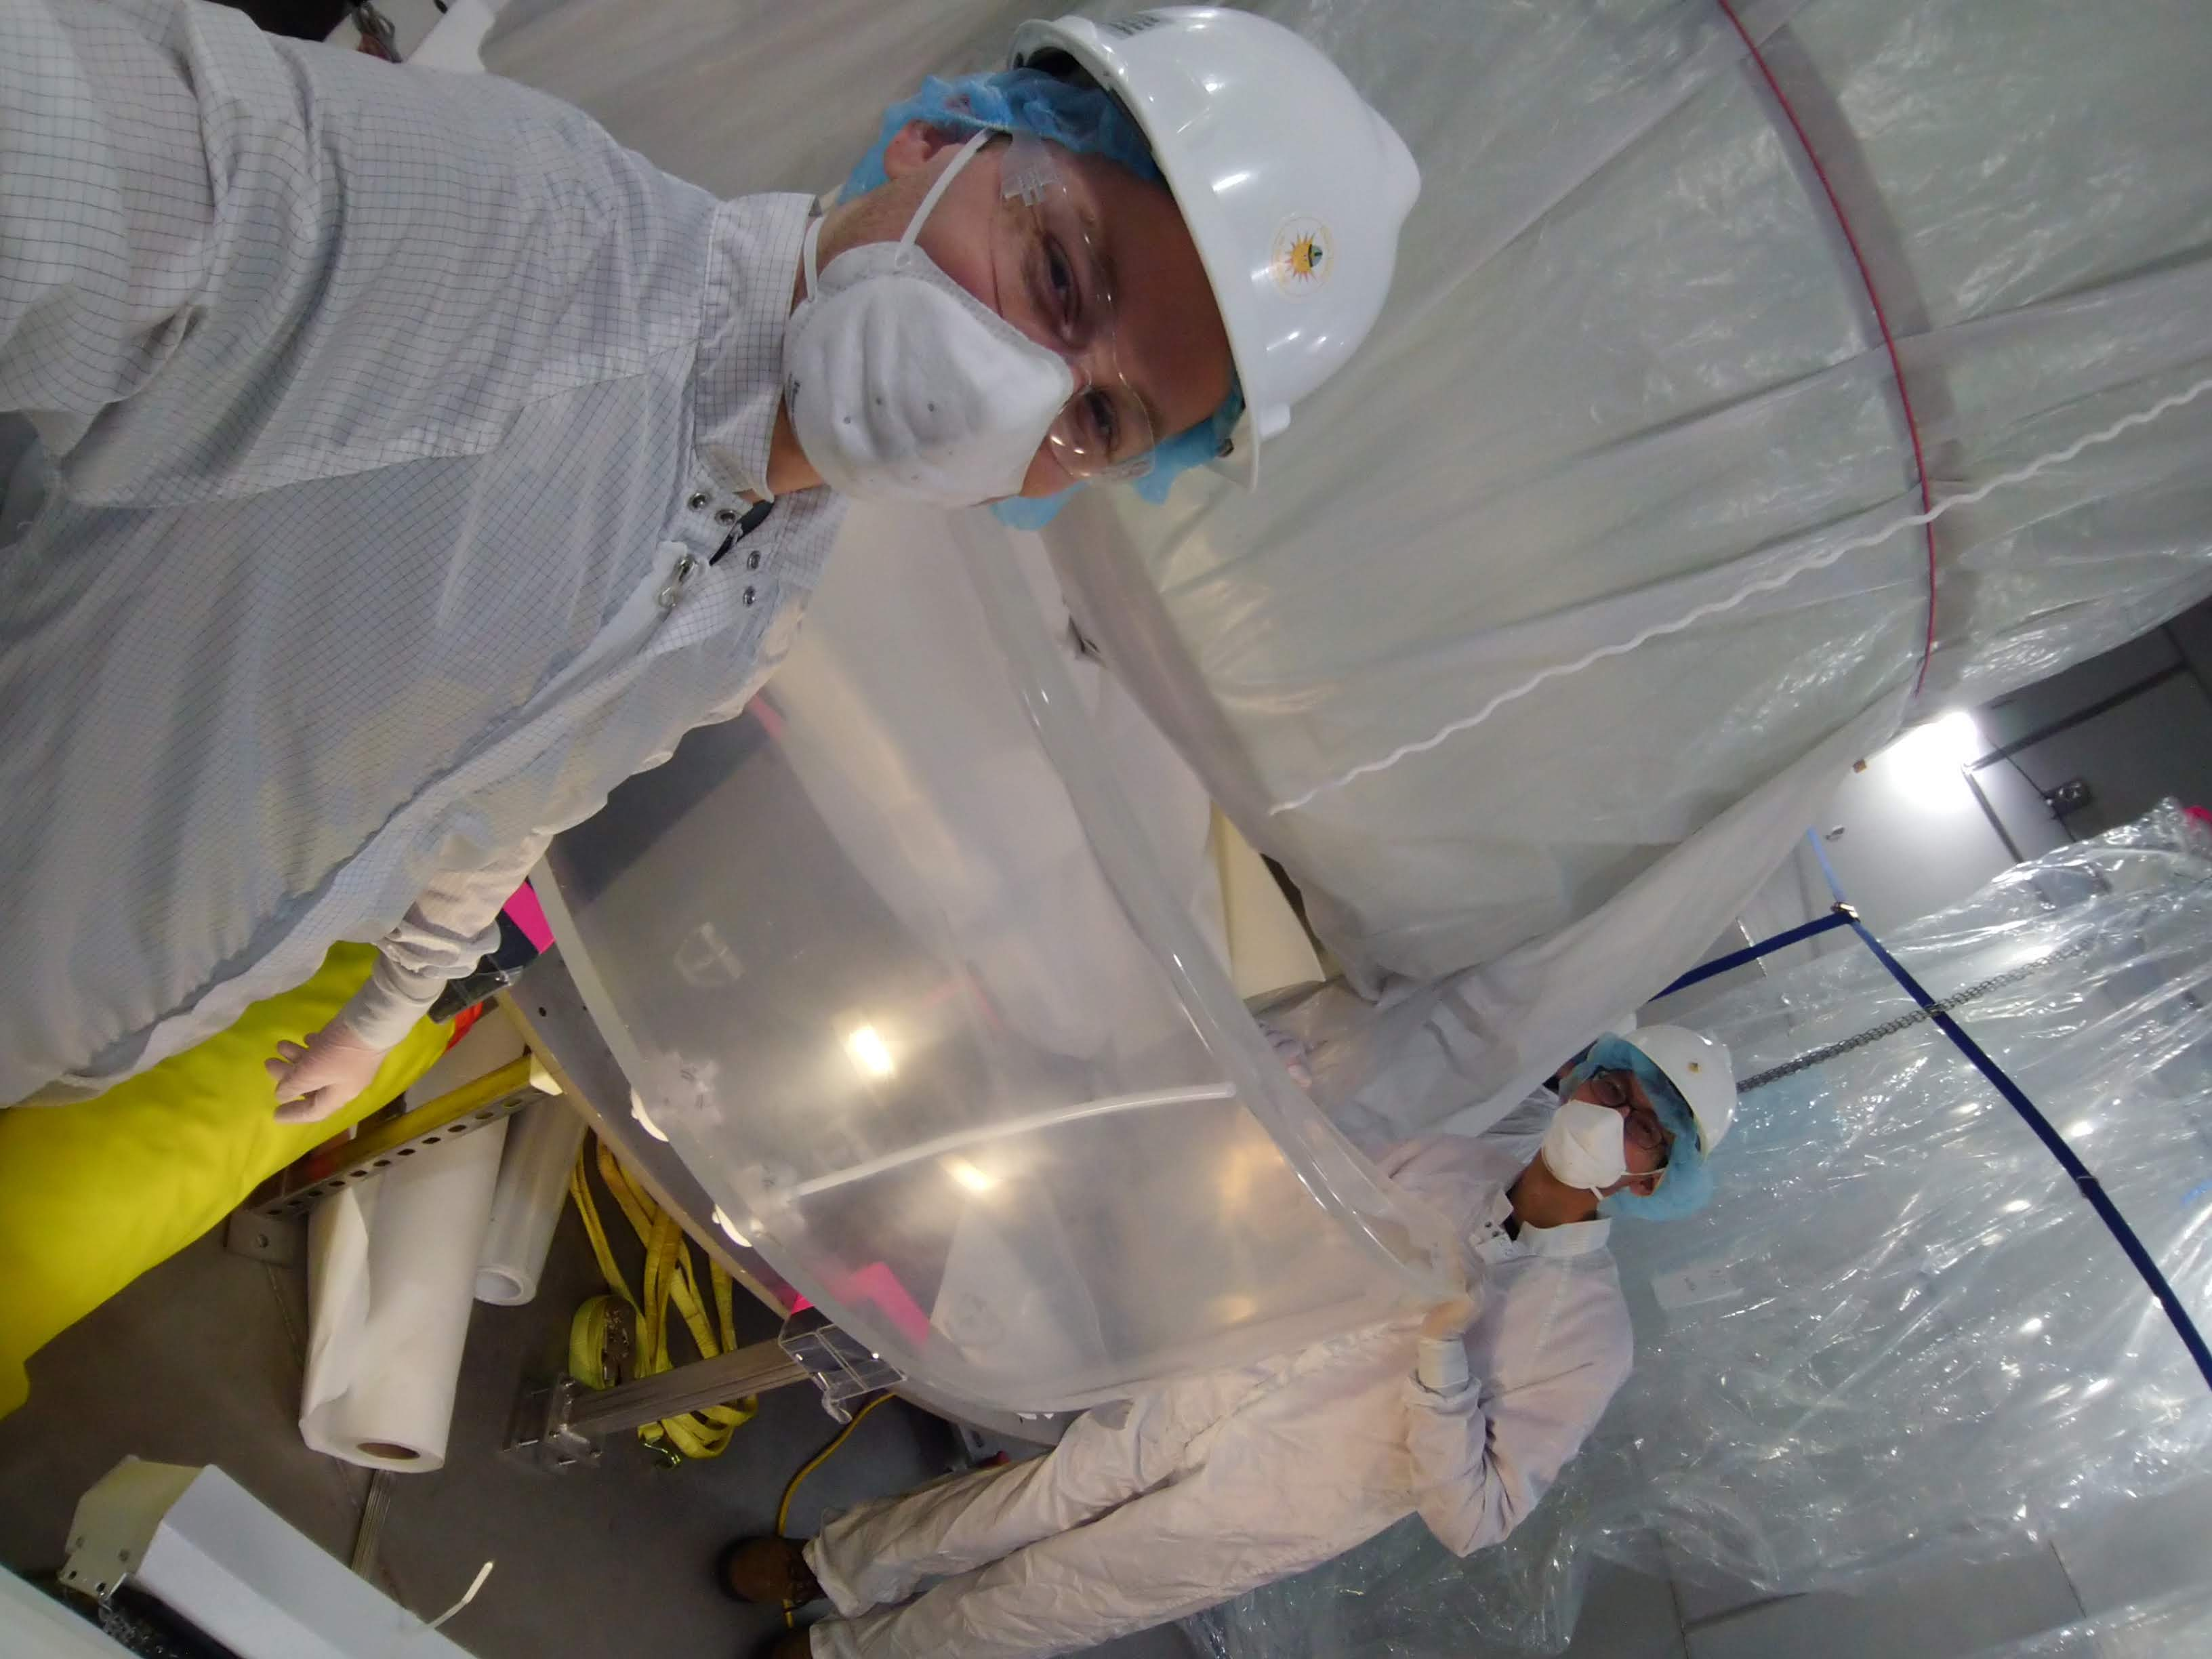
\includegraphics[angle=90, width=\linewidth]{Figures/Construction/BAT_installation.jpg}
  \caption{Installation of the final BAT}
  \label{fig:BAT_installation}
  \end{subfigure}
  \begin{subfigure}{.5\textwidth}
  \centering
  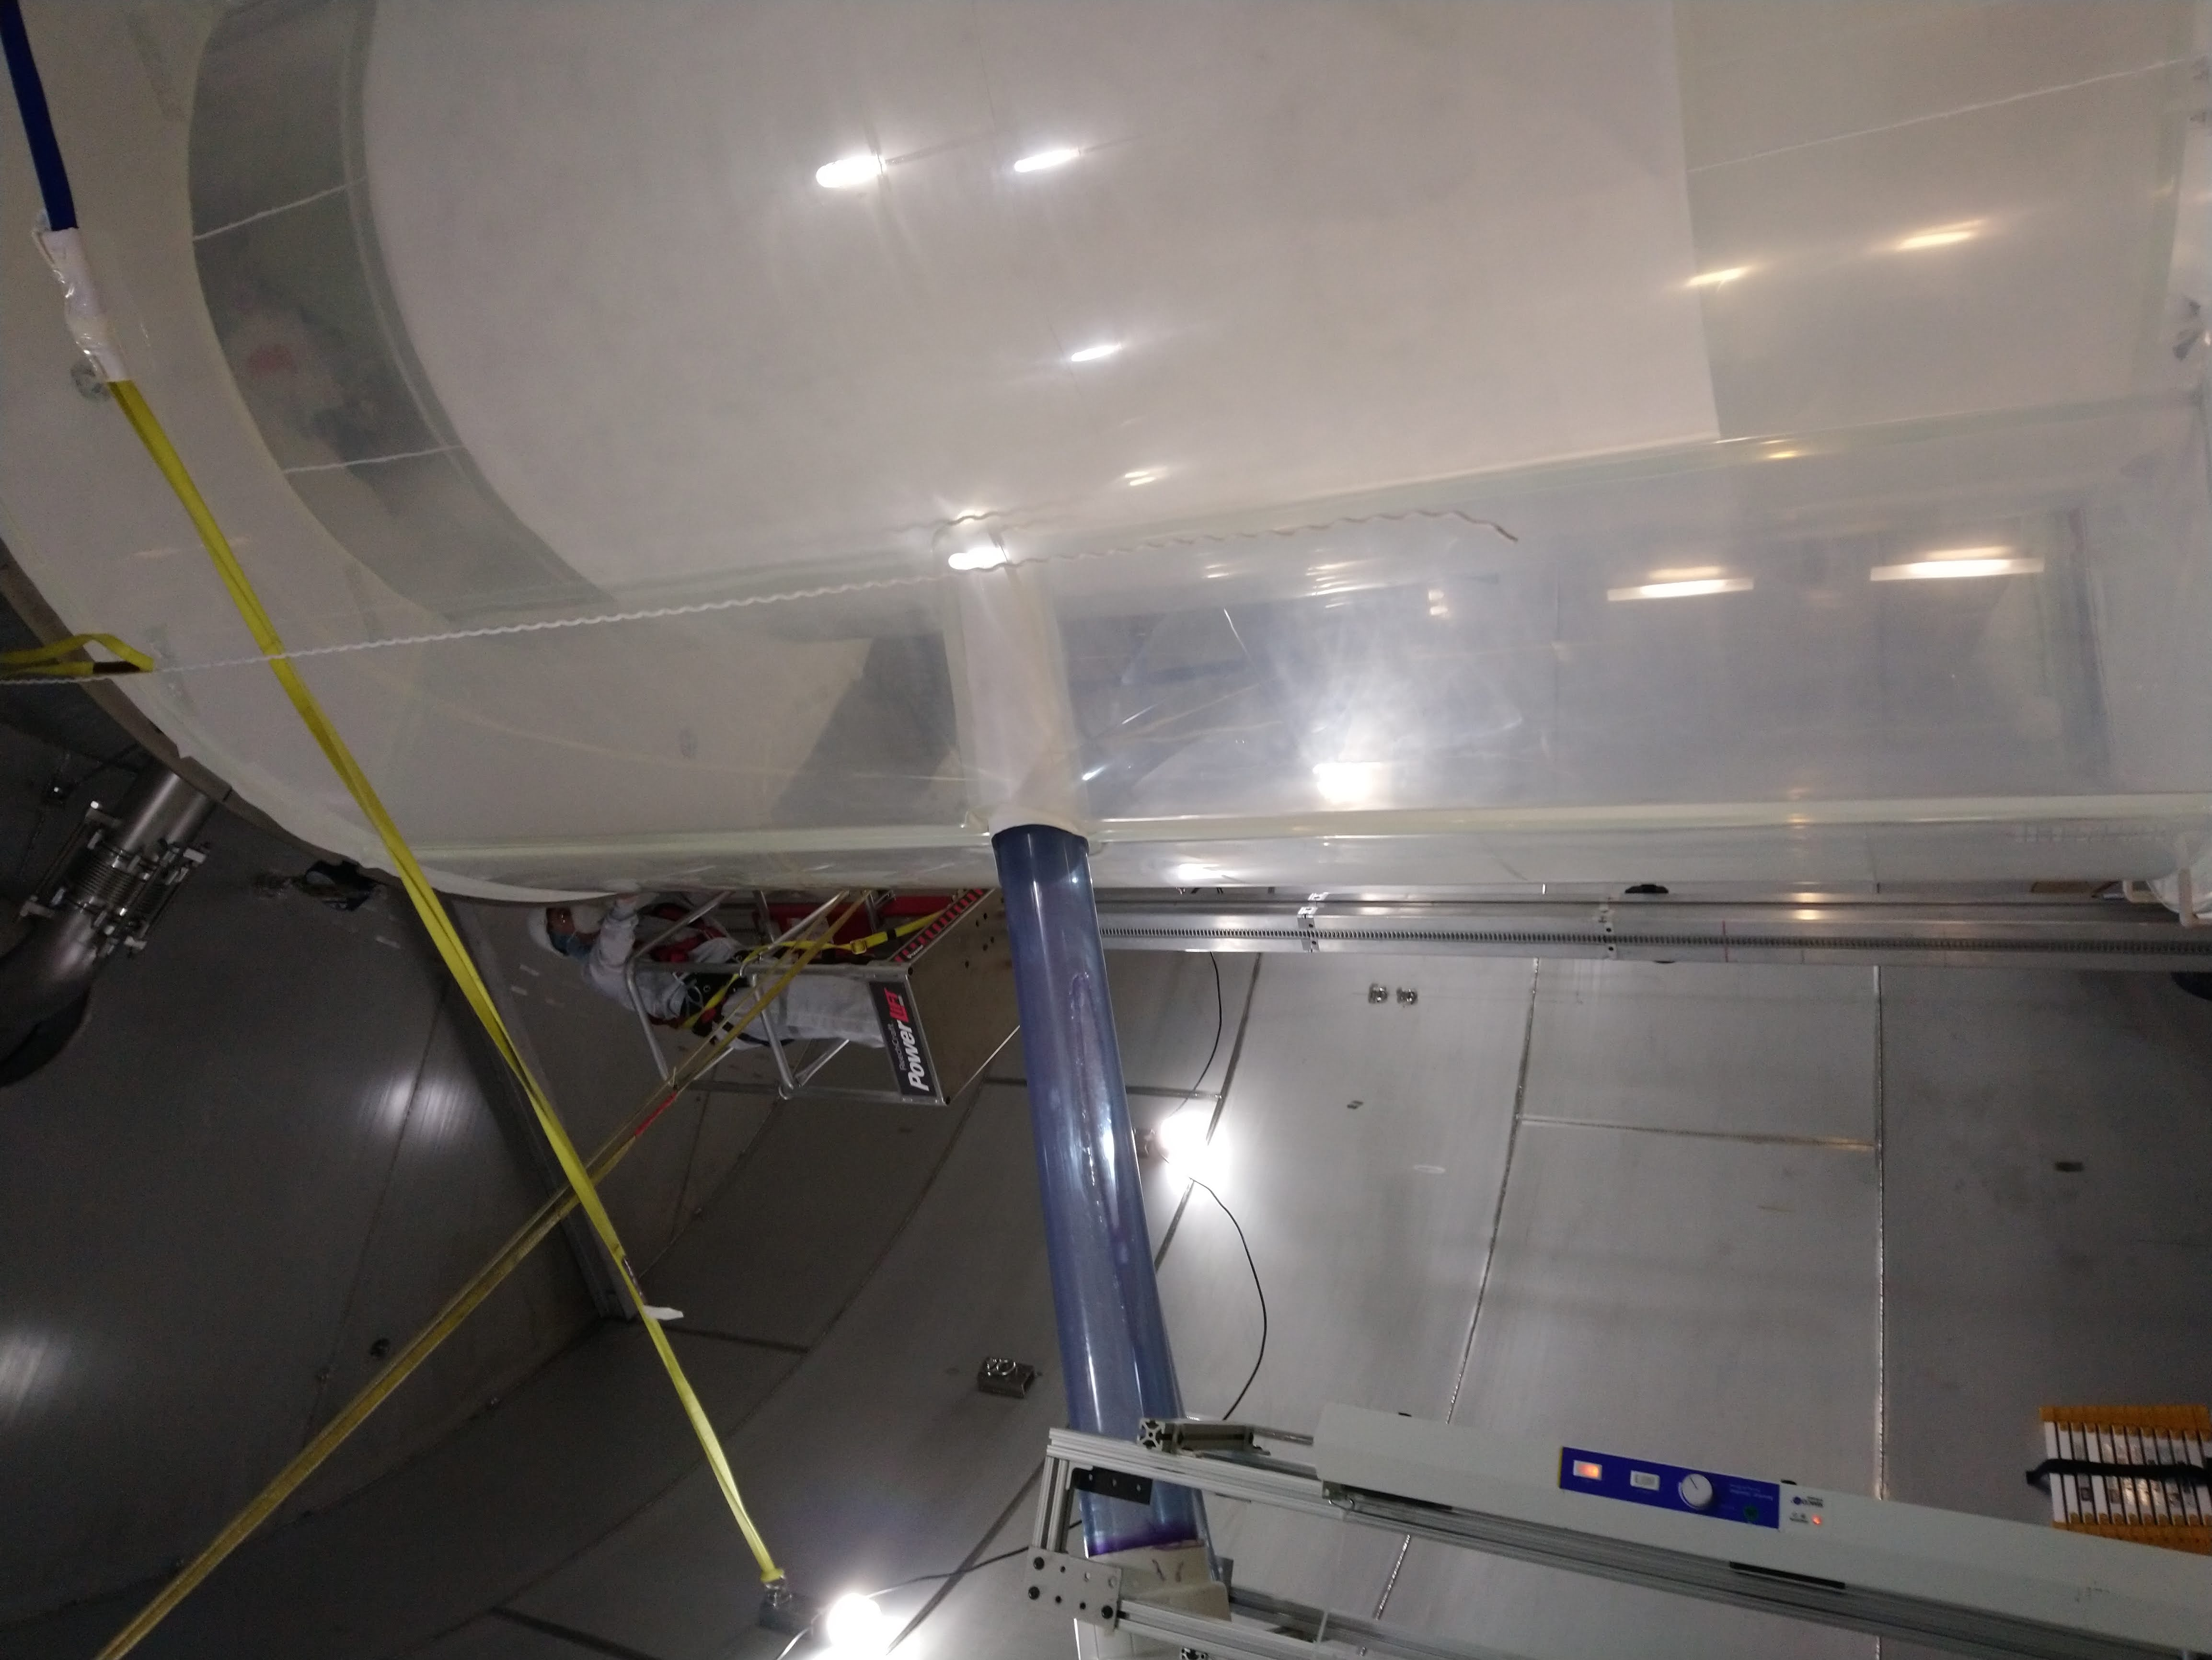
\includegraphics[angle=-90, width=\linewidth]{Figures/Construction/SAT_titanium_plate.JPG}
  \caption{Author securing the SAT.}
  \label{fig:SAT_titanium_installation}
  \end{subfigure}
\caption{Photographs of BAT and SAT installation.}
\label{fig:sat_and_bat_installation}
\end{figure}

\par
In addition to what has been mentioned, the SATs were secured using titanium plates.
To even the load the SATs experience, 1-inch thick polyethylene foam was installed above and below.
Additionally, foam was installed and secured with HandiFoam\textsuperscript{\textregistered} around the High Voltage port, where previously this was just a large gap which would be filled with water.
This is shown in \autoref{fig:hv_port_foam}.

\par
On top of everything, Tyvek was installed, and the PMT ladders were erected around the SATs.
The culmination of all of this is the completed OD, shown in \autoref{fig:complete_od}.
%The use of a single layer will have a performance reduction with the reflectivity reducing by $\approx$10\% compared to multiple layers bonded together \cite{tyvek_reflectivity_ref}.

\begin{figure}[]
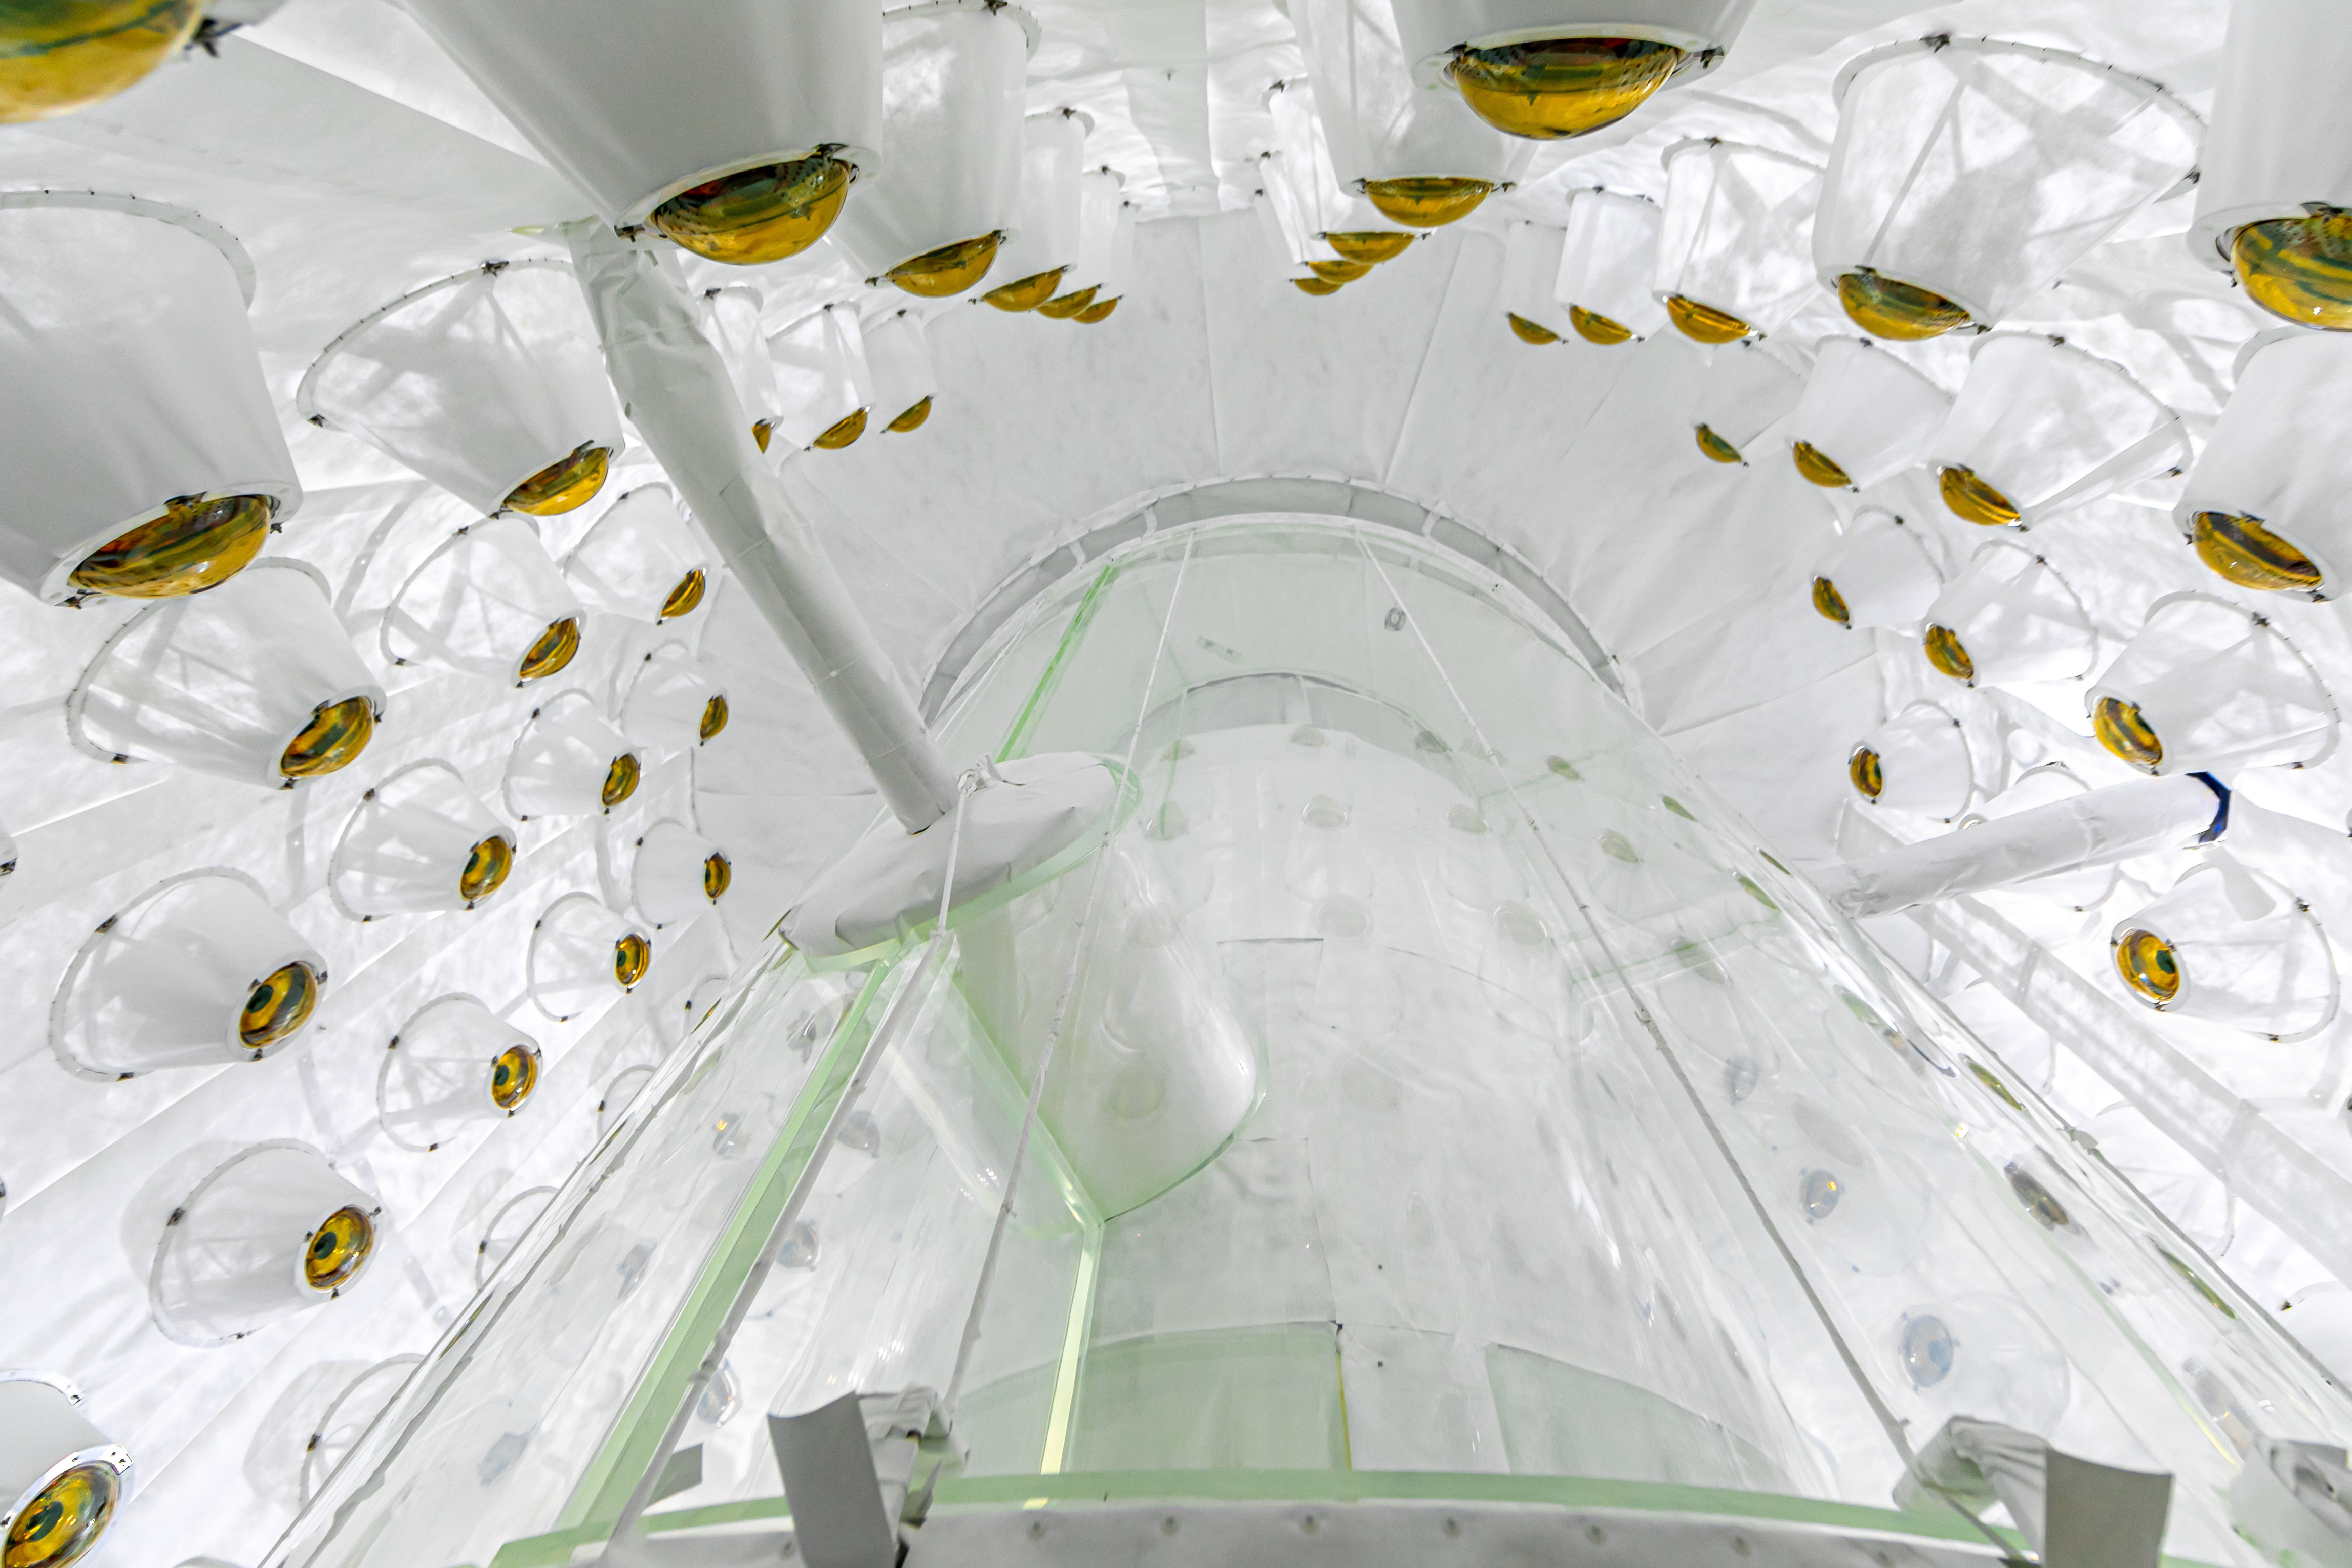
\includegraphics[width=\textwidth]{Figures/Construction/od_complete.jpg}
\centering
\caption{Completed OD installation}
\label{fig:complete_od}
\end{figure}

\par
During the installation described above, the cavern blasting for the Deep Underground Neutrino Experiment (DUNE) began \cite{dune_blasting_ref}.
There was a concern that the pressure change caused by the explosions would damage the tanks.
To stop this, the tanks' valves were opened whenever there was a planned blast.
This left the inside of each tank open to the cavern air, which potentially allowed them to become contaminated.


\subsection{Simulation Adaptation}
\par
Many of these design changes, whether it be material or geometrical, will have some effect on the performance of the OD.
All large changes have been implemented in the simulation: the raised TATs, the additional foam, the Tyvek TeePee, and the change in acrylic thickness.
What is implemented within the simulation can be seen \autoref{fig:Geometry_Differences} where the differences between design and as-built are highlighted.
In black is the desgined geometry and in red are the changes that were described in this section.



\begin{figure}[]
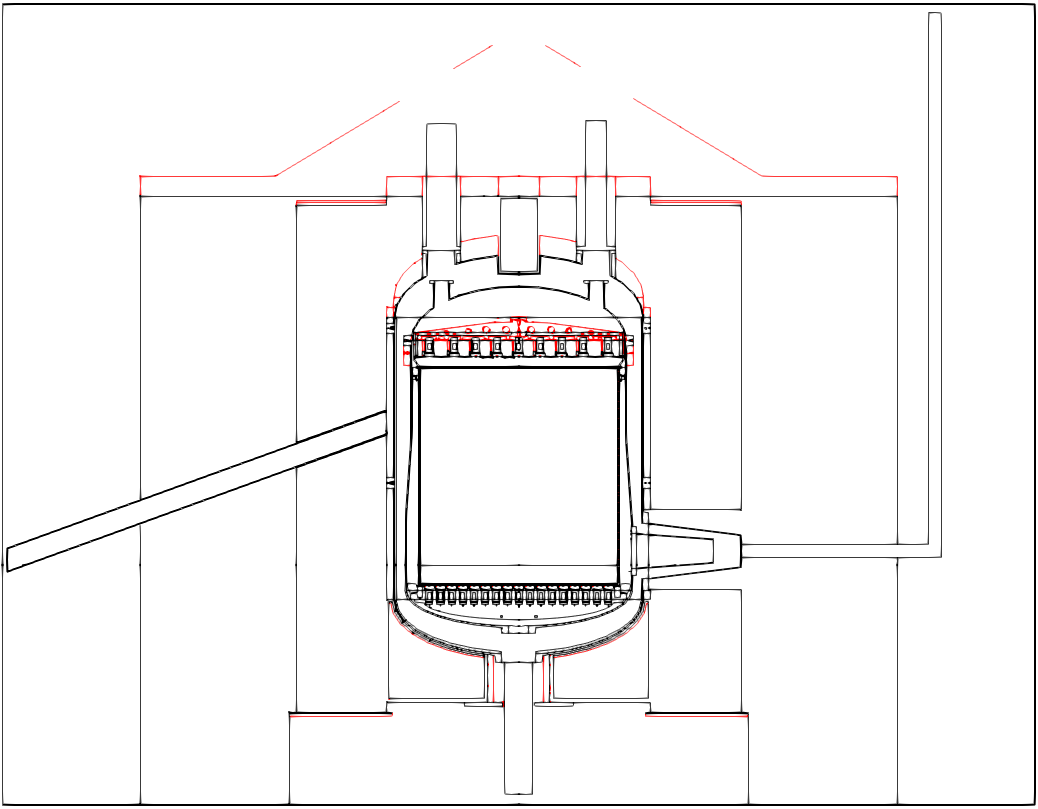
\includegraphics[width=\textwidth]{Figures/Geometry/geometry_differences_black_and_white.png}
\centering
\caption{LZ geometry slice as implemented in Geant4 from the water tank in. In black: the designed geometry as in \autoref{fig:LZ_Cut_CAD}. In Red: changes to the design, including raised Top OD tanks and additional foam. OD PMTs are not shown, as none are in this plane.}
\label{fig:Geometry_Differences}
\end{figure}

%\begin{table}[!htbp]
%    \centering
%    \begin{tabular}{ c | c | c } 
%    \hline
%    \multirow{2}{*}{Volume} & \multicolumn{2}{l}{Percentage captured in volume (\%)} \\ 
%                            & All Neutrons  & SS and FID  \\ \hline
%    volA    & 0.0   & 1232\\
%    volB    & 0.0   &
%    \end{tabular}
%    \caption{Fraction of background neutrons captured in various detector volumes}
%    \label{tab:fraction_of_neutrons_captured_in_volumes}
%\end{table} 